% !TEX encoding = UTF-8
% !TEX TS-program = pdflatex
% !TEX root = ../tesi.tex

%**************************************************************
\chapter{Introduzione ai casi d'uso per l'analisi comparativa}
\label{cap:casi-uso}
%**************************************************************

\intro{Il capitolo descrive in dettaglio il prototipo realizzato e la sua migrazione da REST a GraphQL. A seguire si illustrerà una ulteriore migrazione realizzata sull'applicativo aziendale SushiLab.}\\
%\subsection{Confronto con stakeholder}
\section{Prototipo}
\subsection{Introduzione}
Il prototipo è stato realizzato avendo presente i seguenti obbiettivi:
\begin{itemize}
  \item familiarizzare con le tecnologie Spring e Angular per la realizzazione rispettivamente di backend e frontend;
  \item familiarizzare con la realizzazione delle API sia con lo stile architetturale REST che con il linguaggio di query GraphQL;
  \item avere un caso d'uso ulteriore a conferma delle analisi che verranno poi ricavate dalla migrazione dell'applicativo SushiLab;
\end{itemize}
Si è scelto di realizzare un gestionale server - client in grado di gestire un insieme di impiegati. Ogni impiegato può lavorare in un dipartimento e può dividere il suo tempo su uno o più progetti. Una sede aziendale può contenere uno o più dipartimenti.
\subsection{Architettura ed entità}
\subsubsection*{Architettura generale dell'applicativo}
L'applicativo segue l' architettura raffigurata nell'immagine \ref{prototype-architecture}. Il backend del prototipo è stato realizzato con framework Spring Boot mentre il frontend con framework Angular.
\FloatBarrier
\begin{figure}[!h]
\centering
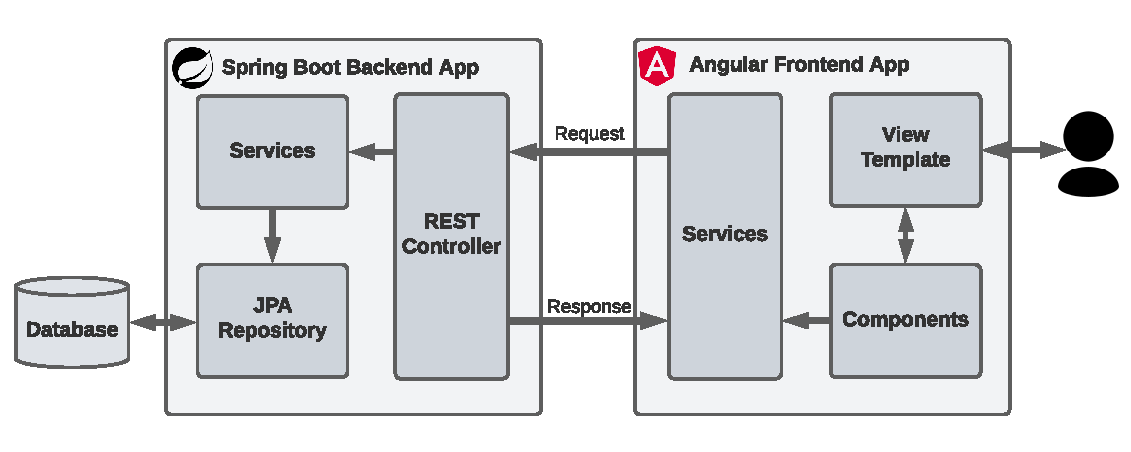
\includegraphics[width=1\linewidth]{immagini/prototypeArchitecture.pdf}
\caption{Architettura del prototipo di Web Application.}
\label{prototype-architecture}
\end{figure}
\FloatBarrier
Le richieste effettuate dai servizi del client vengono mappate sul REST controller del server il quale, dopo la rielaborazione interna delle richiesta, ritorna la risposta al client; quest'ultimo può dunque aggiornare la vista visualizzata dall'utente. In seguito vengono affrontati più nel dettaglio i moduli interni sia per quanto riguarda il server che il client.
\subsubsection*{Entità e relazioni}
\label{entity-relation}
Trattandosi di un gestionale aziendale semplificato si prevedono solo quattro entità principali:
\begin{itemize}
  \item \textbf{Employee}: l'impiegato che può lavorare ad uno o più progetti e in un dipartimento;
  \item \textbf{Project}: un progetto aziendale a cui partecipano più impiegati;
  \item \textbf{Site}: la sede aziendale, può avere più dipartimenti;
  \item \textbf{Department}: un dipartimento che appartiene ad una sede.
\end{itemize}
Ciascuna entità è caratterizzata dai campi presenti in figura \ref{ER-prototype}. I campi in grassetto rappresentano la chiave primaria, quelli sottolineati le chiavi esterne. Le relazioni presenti tra le varie entità sono:
\begin{itemize}
  \item \textbf{many to many}: è presente tra Employee e Project, infatti ciascun impiegato può lavorare a più progetti e ciascun progetto può avere più impiegati; viene scomposta in due relazioni \textit{one-to-many} con la tabella \textit{Employees\_Projects};
  \item \textbf{one to many}: è presente in due situazioni:
  \begin{itemize}
    \item tra Employee e Department, infatti ciascun impiegato deve lavorare almeno in un dipartimento, mentre ciascun dipartimento può ospitare più impiegati;
    \item tra Department e Site, ciascun dipartimento può appartenere esclusivamente ad una sede, mentre ciascuna sede può esser composta da più dipartimenti.
  \end{itemize}
\end{itemize}
%%% IMG
\FloatBarrier
\begin{figure}[!ht]
\centering
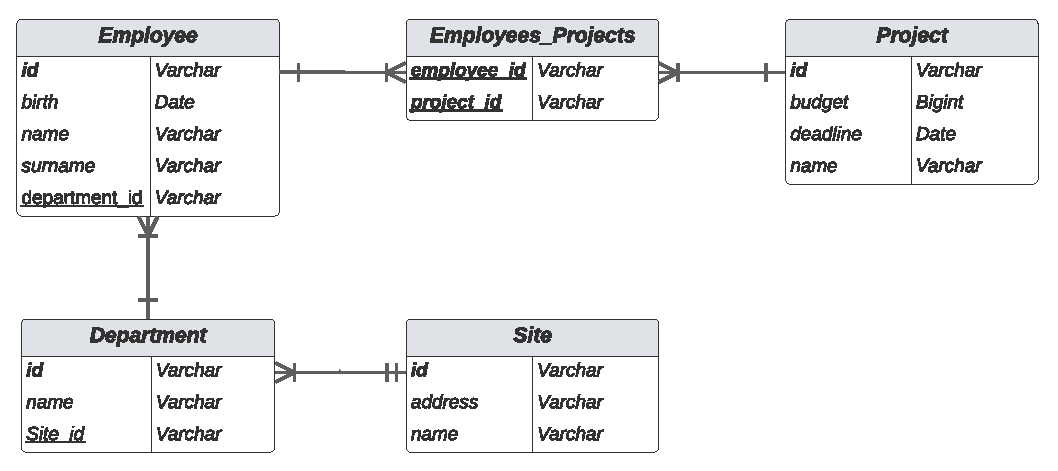
\includegraphics[width=1\linewidth]{immagini/ER_prototype.pdf}
\caption{Schema ER delle entità del prototipo.}
\label{ER-prototype}
\end{figure}
\FloatBarrier
%%% IMG
\subsection{Progettazione e realizzazione backend}
\subsubsection*{Architettura backend}
È stato deciso di seguire il pattern \textbf{controller - service - repository} per la realizzazione del server del prototipo.  Il pattern rispetta perfettamente il principio di "Separation Of Concerns". Di seguito in figura \ref{controller-service-repository} è possibile visualizzare l'architettura del backend.
%%%% IMG
\FloatBarrier
\begin{figure}[!h]
\centering
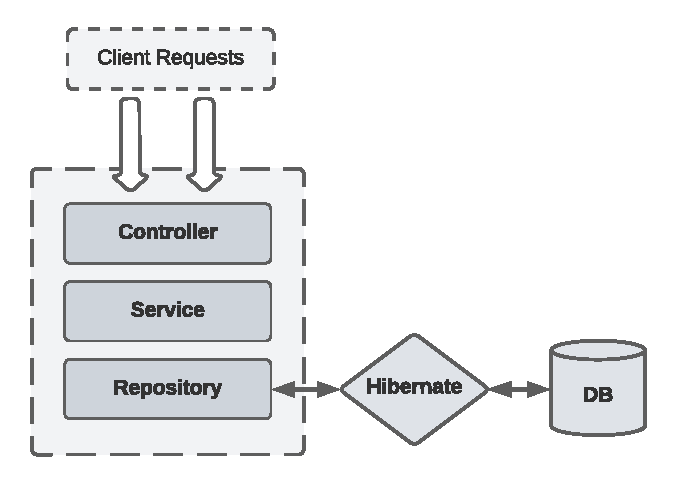
\includegraphics[width=0.8\linewidth]{immagini/controllerServiceRepository.pdf}
\caption{Architettura interna backend.}
\label{controller-service-repository}
\end{figure}
\FloatBarrier
%%%% IMG
Nell'immagine \ref{sequence-diagram} è possibile visualizzare il diagramma di sequenza di una richiesta GET al server da parte del client. La richiesta in questo caso è andata a buon fine ritornando al client i dati richiesti.
\FloatBarrier
\begin{figure}[!h]
\centering
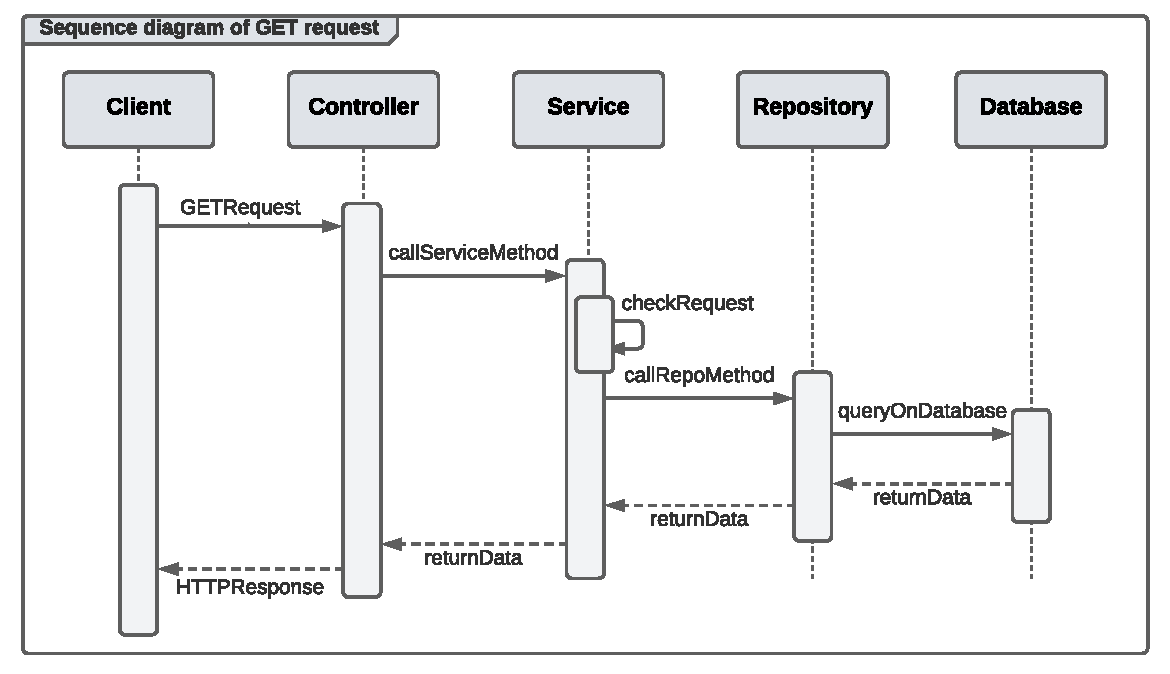
\includegraphics[width=1\linewidth]{immagini/getRequestFromClient.pdf}
\caption{Diagramma di sequenza di una richiesta GET elaborata dal server.}
\label{sequence-diagram}
\end{figure}
\FloatBarrier
Il pattern prevedere la gestione delle entità e delle chiamate alle API attraverso tre strati:
\begin{itemize}
  \item \textbf{Controller layer}: è l'unico responsabile della comunicazione con i client, inoltre gestisce le interfacce REST e invoca lo strato di servizio;
  \item \textbf{Service layer}: è lo strato tra controller e repository, si occupa della business logic e qualora sia necessario visualizzare, salvare, modificare o eliminare dati allora comunica con lo strato di persistenza;
  \item \textbf{Repository layer}: si tratta dello strato inferiore dell'architettura, si occupa della gestione dei dati e delle loro modifiche nonché della gestione del database.
\end{itemize}
Durante la realizzazione viene seguito il percorso inverso rispetto a quanto visto nell'immagine \ref{controller-service-repository}: la realizzazione avviene partendo dallo strato di persistenza, dunque dalla creazione delle entità e del livello di repository.
\subsubsection*{Entità e repository}
A ciascuna entità del database viene fatta corrispondere una classe in Java quindi sono state realizzate quattro classi rappresentanti le entità Employee, Project, Department e Site.\\
Ciascuna classe implementa la classe \textit{Serializable}, così facendo è possibile serializzare i dati in flussi di byte. La serializzazione viene utilizzata poiché si tratta di dati che dovranno essere memorizzati nel database, è necessario serializzarli poiché abbandonano la Java Virtual Machine. Viene inoltre utilizzato un \textit{serialVersionUID} per attribuire una versione a ciascuna classe serializzabile in modo da garantire la consistenza delle classi memorizzate in banca dati.\\
Di seguito l'esempio dell'implementazione della classe Employee:
%%% IMG
\FloatBarrier
\begin{figure}[!ht]
\centering
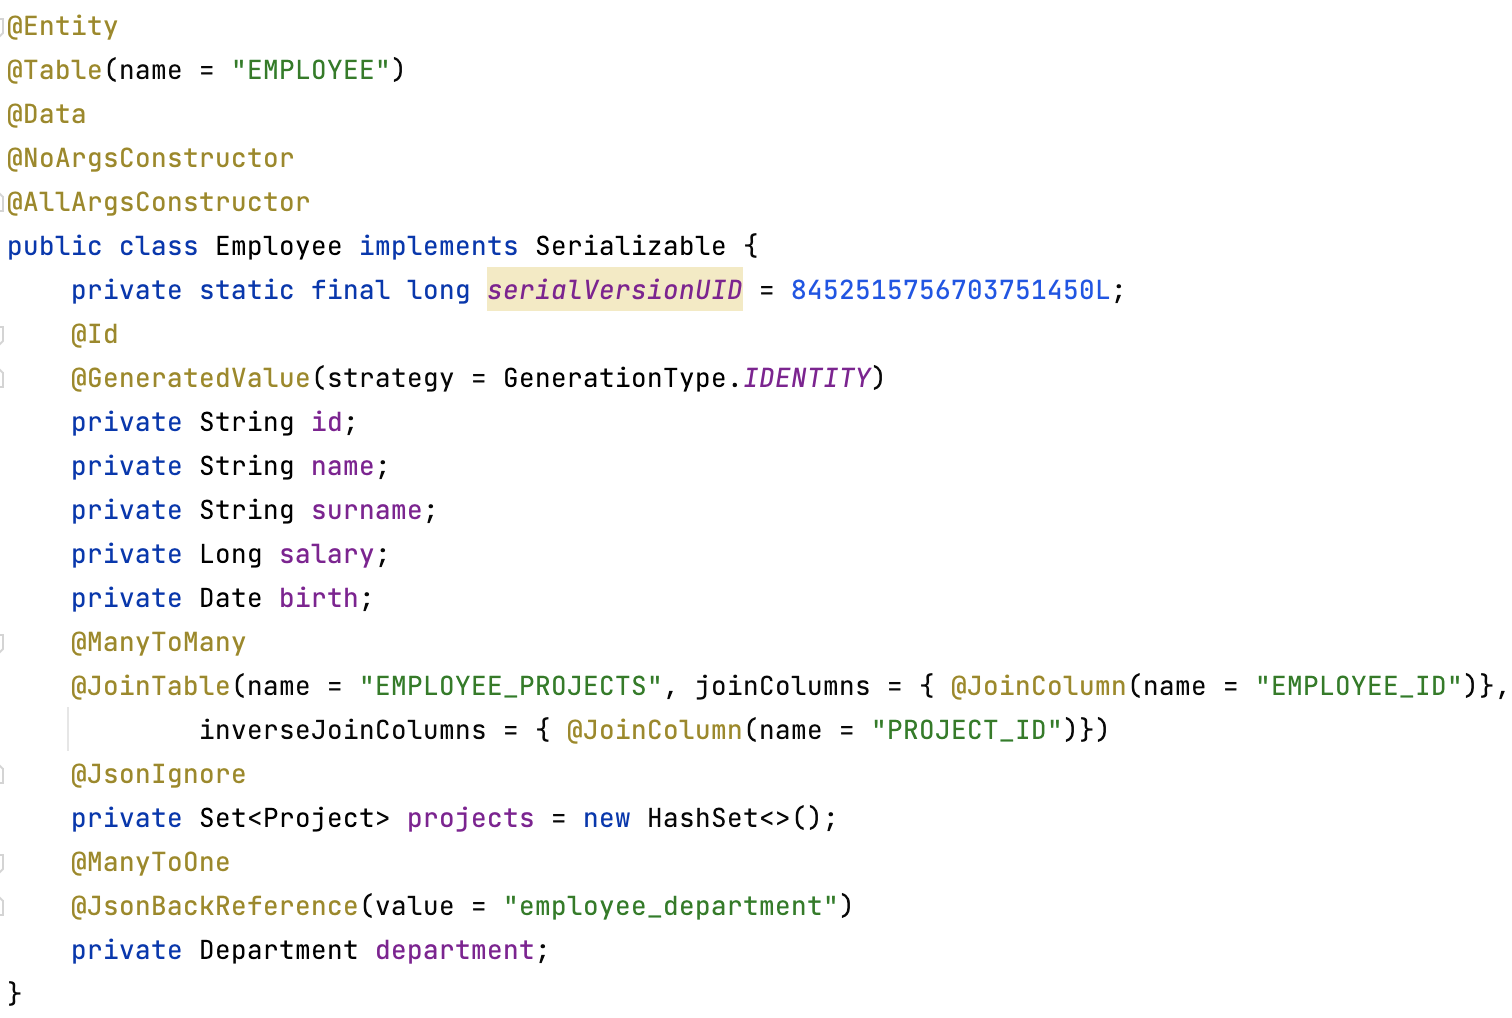
\includegraphics[width=0.9\linewidth]{immagini/employee_entity.png}
\caption{Esempio di implementazione dell'entità Employee in Spring Boot.}
\label{employee-entity-definition}
\end{figure}
\FloatBarrier
%%% IMG
Vengono attribuite alla classe Employee diverse annotazioni Spring, tra queste:
\begin{itemize}
  \item \textbf{@Entity}: si tratta dell'annotazione che permette di mappare la classe Employee come tabella nel database. Questa annotazione è resa disponibile dal modulo Spring Data JPA il quale implementa la specifica delle Java Persistence API attraverso Hibernate ORM e permette dunque il mapping della classi con corrispettive entità nel database;
  \item \textbf{@Table}: questa annotazione permette di specificare il nome della tabella generata o presente nel database durante la sua creazione o aggiornamento;
  \item \textbf{@Data}: grazie alla libreria \textit{lombok} è possibile, attribuendo alla classe questa annotazione, generare automaticamente tutti i metodi get e set per ciascun campo della classe;
  \item \textbf{@NoArgConstructor e @AllArgConstructor}: permettono di generare tutte le combinazioni di costruttori con e senza parametri.
\end{itemize}
Le annotazioni applicate agli attributi della classe sono:
\begin{itemize}
  \item \textbf{@Id}: associato al campo \textit{id}, specifica durante il mapping che si tratta della chiave primaria;
  \item \textbf{@GeneratedValue}: associato al campo \textit{id}, specifica che quando una nuova istanza dell'entità viene creata, deve essere generato un nuovo id randomico;
  \item \textbf{@ManyToMany} e \textbf{@ManyToOne}: queste specificano il tipo di relazione che è presente con le altre entità, sono rispettivamente associate ai campi \textit{projects}, con il quale Employee ha una relazione molti a molti e infine al campo \textit{department}, con il quale Employee ha una relazione molti a uno;
  \item \textbf{@JoinTable}: è associata al campo \textit{projects}, e poiché le relazioni molti a molti necessitano di una ulteriore tabella per la memorizzazione di tutte le associazioni, questa annotazione permette di specificarne il nome, ovvero \textit{EMPLOYEE\_PROJECTS} e i nomi delle due colonne, ovvero \textit{EMPLOYEE-ID} e \textit{PROJECT-ID};
  \item \textbf{@JsonIgnore}: associato al campo \textit{projects}, permette di escluderlo dalla serializzazione;
  \item \textbf{@JsonBackReference}: associato al campo \textit{department}, permette di dare una direzionalità alla relazione molti a uno con Department, fondamentale per evitare il problema della ricorsione infinita.
\end{itemize}
Analogamente sono state realizzate le classi corrispondenti alle entità Project, Department e Site.\\\\
A questo punto si procede con la realizzazione delle classi repository: ciascuna entità ha una propria repository corrispondente. Viene estesa l'interfaccia \textbf{JPArepository<T, ID>} con T il tipo della entità che si vuole gestire, mentre ID è il tipo della chiave primaria dell'entità T. La repository JPA estende le seguenti interfacce:
\begin{itemize}
  \item \textbf{CrudRepository<T, ID>}: contiene i metodi per gestire le classiche operazioni CRUD;
  \item \textbf{PagingAndSortingRepository<T, ID>}: contiene i metodi per gestire la paginazione e l'ordinamento;
\end{itemize}
Estendendo la JPARepository per ciascun tipo è possibile avere a disposizione diversi metodi per eseguire operazioni già implementate come: findAll, count, existById, SaveAndFlush, ecc...\\
Per realizzare ulteriori metodi è sufficiente rispettare le corretta sintassi del nome del metodo affinché Spring si occupi in automatico della sua implementazione.\\
Nel caso in cui si voglia realizzare una query personalizzata si utilizza l'annotazione \textbf{@Query} alla quale è possibile passare come attributo la query che desideriamo in linguaggio JPQL. In figura \ref{employee-repository} un esempio di quanto appena detto:
%%% IMG
\FloatBarrier
\begin{figure}[!ht]
\centering
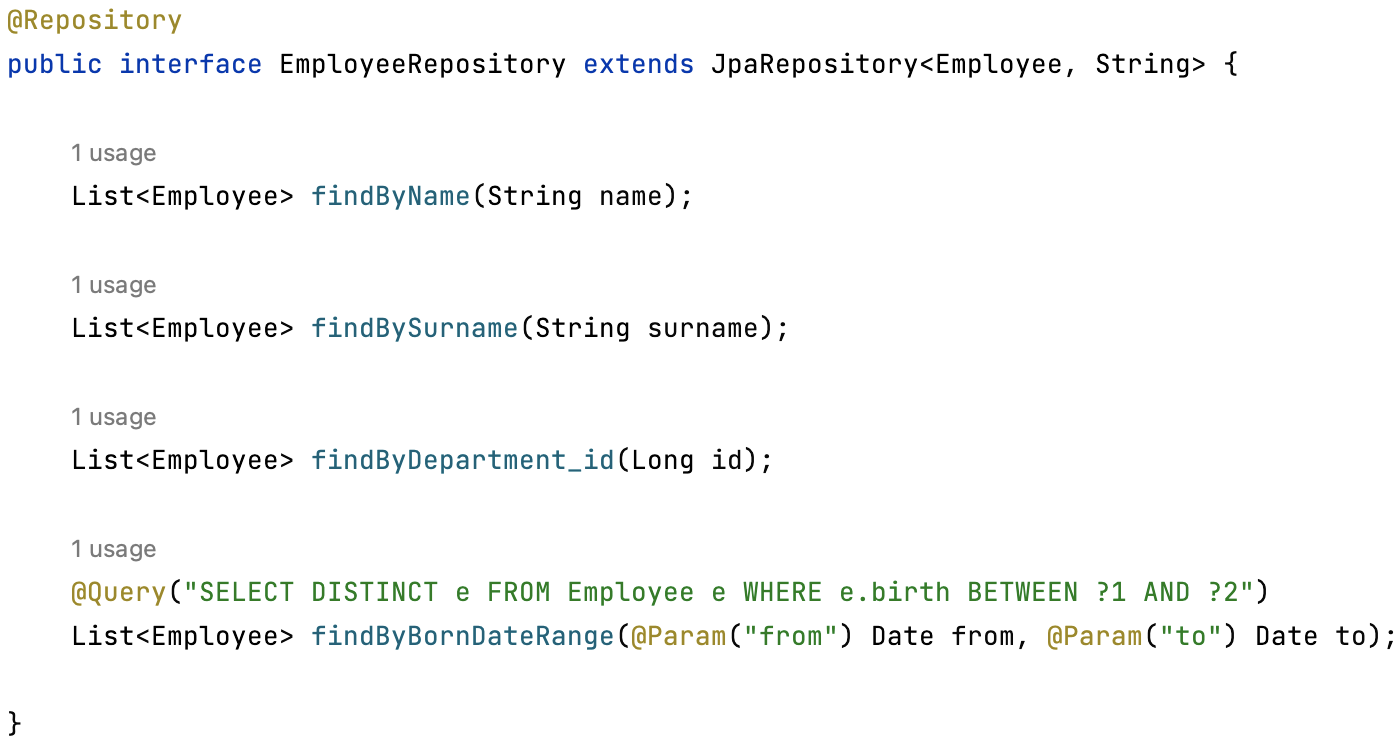
\includegraphics[width=1\linewidth]{immagini/employee_repository.png}
\caption{Esempio di implementazione della repository di Employee in Spring Boot.}
\label{employee-repository}
\end{figure}
\FloatBarrier
%%% IMG
Oltre ai classici metodi di ricerca disponibili sono stati realizzati alcuni metodi per la ricerca di impiegati per nome, per cognome e per id di dipartimento in cui lavorano. Infine è stata realizzata una query personalizzata per la ricerca di impiegati nati in un range di date.\\
Da evidenziare l'uso dell'annotazione \textbf{@Repository} attribuita alla'interfaccia, fondamentale al fine di indicare che la classe fornisce meccanismi per modellare i dati del database.
\subsubsection*{Service}
Il compito dello strato di servizio è facilitare la comunicazione tra controller e repository oltre a realizzare la business logic dell'applicativo.\\
Per ciascun repository, dunque per ciascuna entità, è stato realizzato un servizio specifico per gestirne le logiche.\\
Al fine di rispettare i principi SOLID della programmazione, per questioni di loose coupling, IoC e semplicità nel testing, è stato scelto di implementare il pattern secondo il quale per ogni entità viene realizzata una interfaccia del corrispondente servizio e sua relativa implementazione. In figura \ref{service-serviceImpl} relativo all'entità Employee.
%%% IMG
\FloatBarrier
\begin{figure}[!ht]
\centering
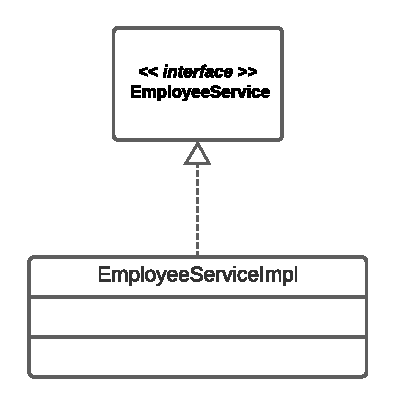
\includegraphics[width=0.3\linewidth]{immagini/service_serviceImpl.pdf}
\caption{Esempio di implementazione dell'interfaccia EmployeeService.}
\label{service-serviceImpl}
\end{figure}
\FloatBarrier
%%% IMG
Di seguito (fig. \ref{employeeServiceImpl}) viene riportato l'esempio dell'implementazione del servizio \textbf{EmployeeServiceImpl}.
%%% IMG
\FloatBarrier
\begin{figure}[!ht]
\begin{mdframed}
\centering
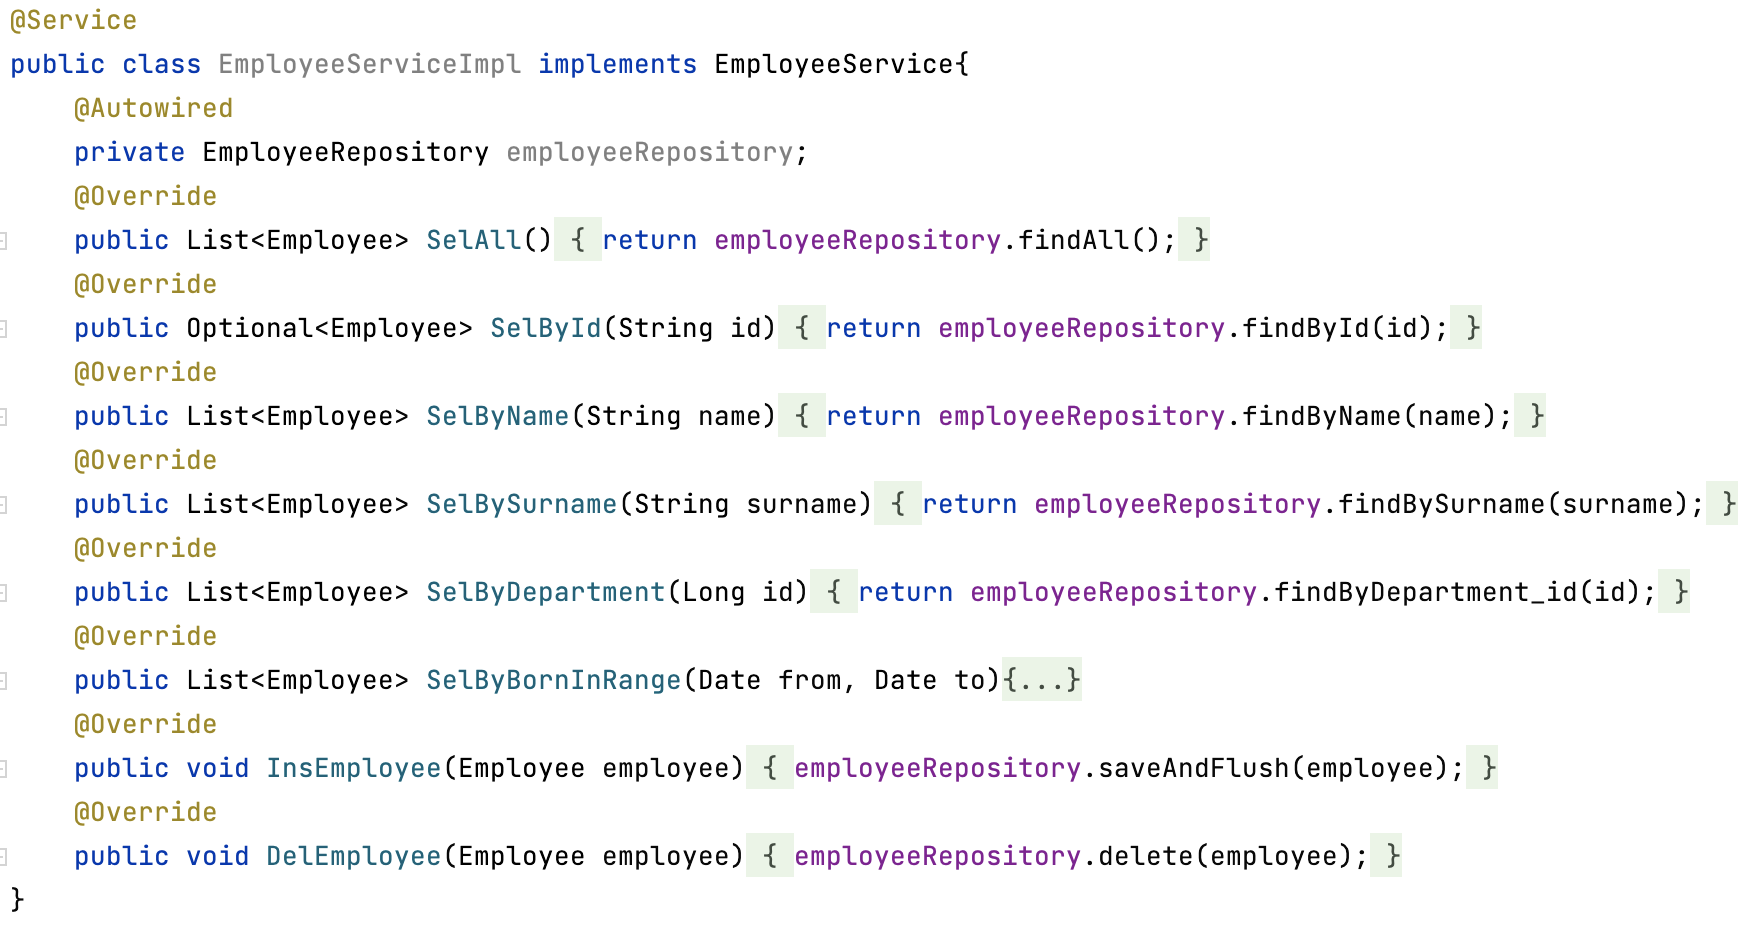
\includegraphics[width=1\linewidth]{immagini/employeeServiceImpl.png}
\end{mdframed}
\caption{Classe EmployeeServiceImpl.}
\label{employeeServiceImpl}
\end{figure}
\FloatBarrier
%%% IMG
In figura \ref{employeeServiceImpl} è possibile notare come la classe sia caratterizzata dall'annotazione \textbf{@Service} la quale viene utilizzata per indicare classi che contengono la business logic e per marcare la classe come service provider.\\\\
Le annotazioni utilizzate sono:
\begin{itemize}
  \item \textbf{@Autowired}: attribuita al campo \textit{employeeRepository} produce la dependency injection della repository \textit{EmployeeRepository} nel servizio;
  \item \textbf{@Override}: utilizzata da tutti i metodi, avverte che i metodi dichiarati nell'interfaccia vengono implementati;
\end{itemize}
Sono stati resi disponibili metodi semplici che vanno ad invocare, grazie alla dipendenza con la repository, le query già disponibili con la \textit{JPARepository<T, ID>} e la query vista precedenemente \textit{SelByBornInRage}.\\
Lo strato di servizio si incarica della gestione delle eccezioni estendendo il gestore  \textit{HandlerExceptionResolver}; in questo modo si migliora il comportamento di default che non sempre fornisce informazioni comprensibili sulla natura dell'errore.
\subsubsection*{Controller}
Lo strato di controller si occupa di gestire le richieste che il server riceve attraverso il protocollo HTTP e di mapparle inoltre sui metodi corrispondenti. In figura \ref{employeeController} il controller di Employee, ovvero la classe \textit{EmployeeController}:
\FloatBarrier
\begin{figure}[!ht]
\begin{mdframed}
\centering
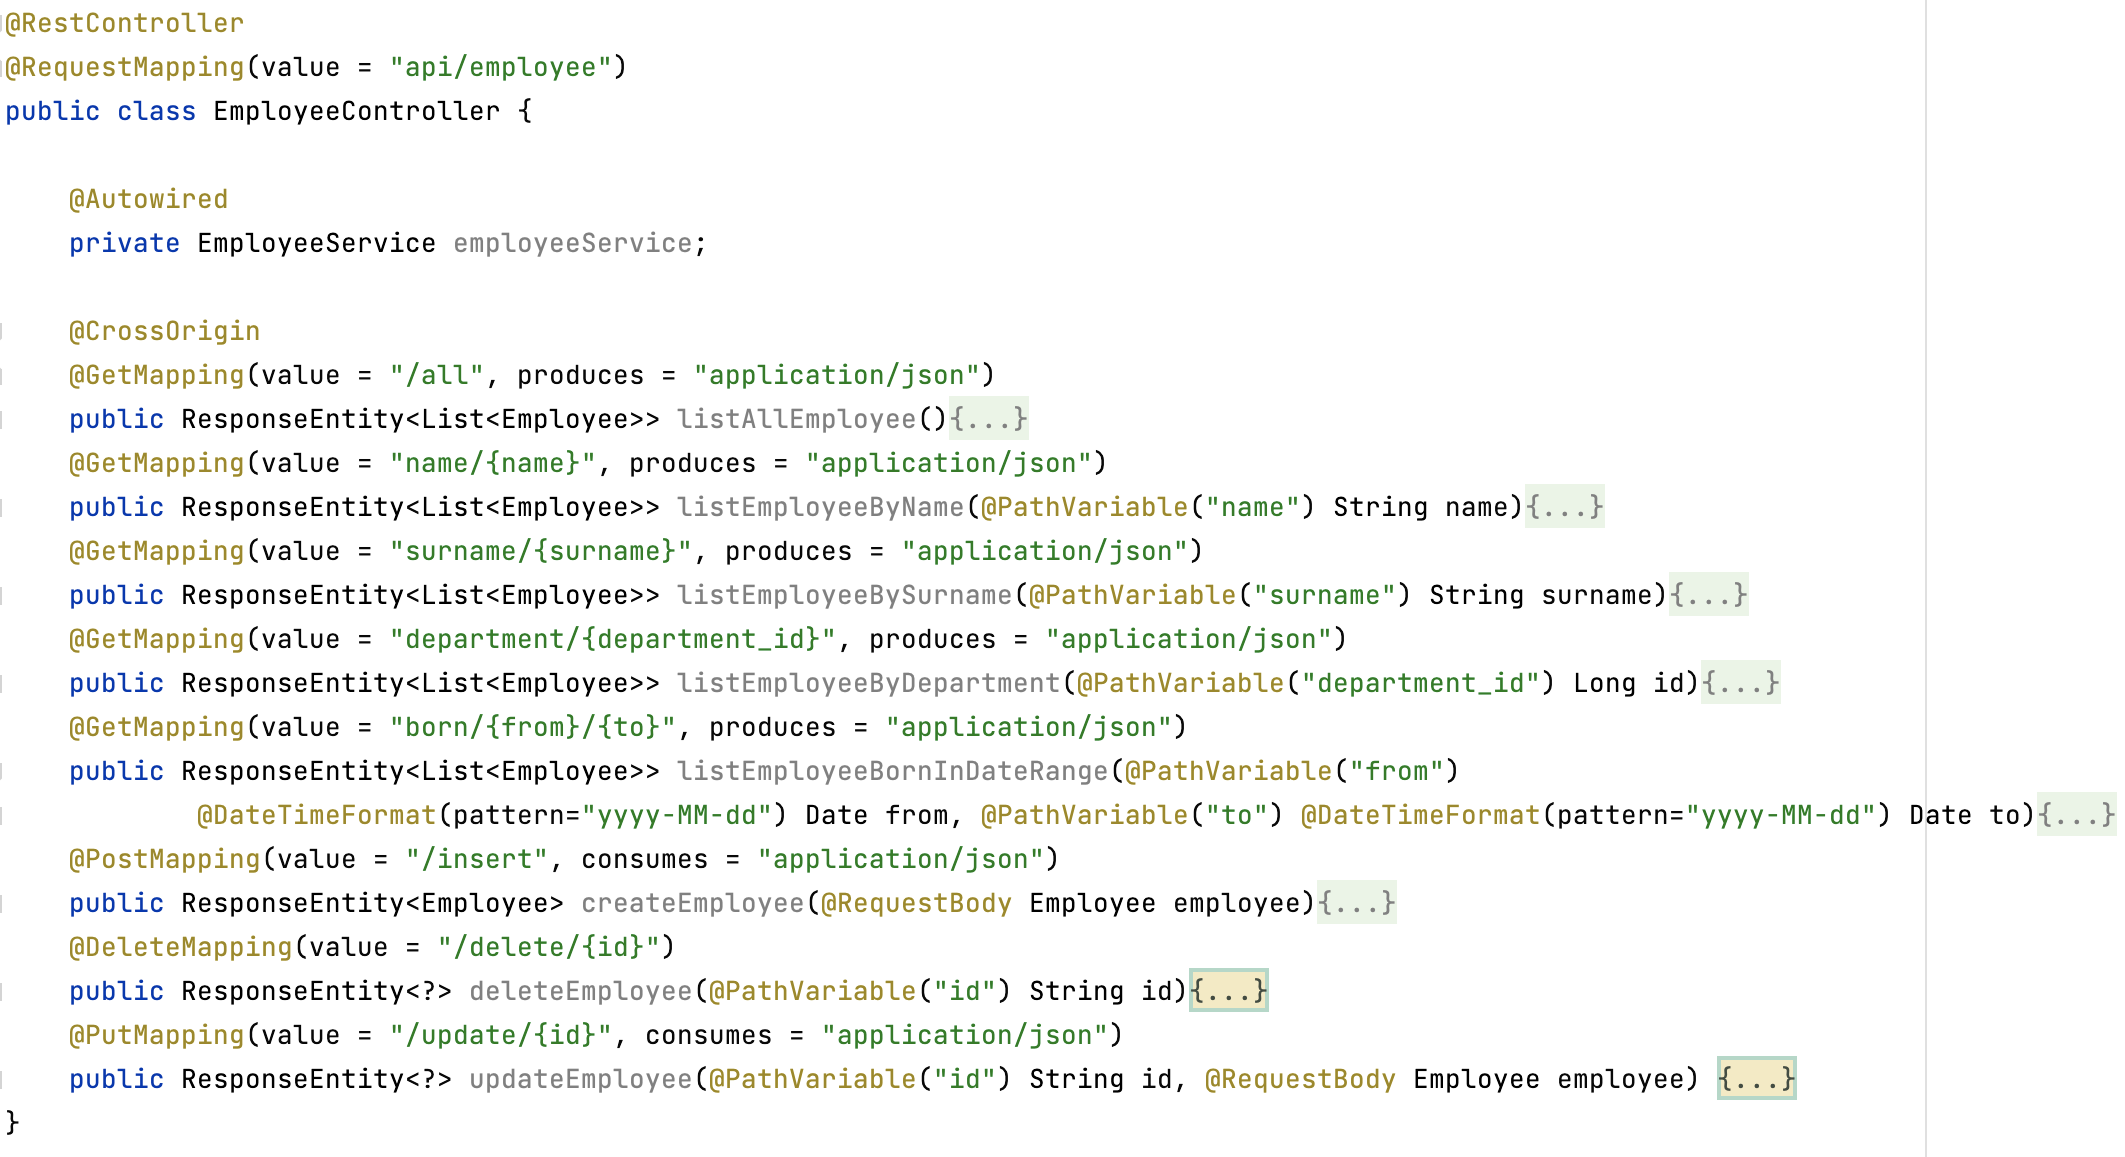
\includegraphics[width=1\linewidth]{immagini/EmployeeController.png}
\end{mdframed}
\caption{Classe EmployeeController.}
\label{employeeController}
\end{figure}
\FloatBarrier
Questa classe permette di gestire e mappare le richieste a seconda dell'url dal quale proviene la richiesta. Di seguito le annotazioni associate alla classe:
\begin{itemize}
  \item \textbf{@RestController}: definisce la classe come controller di tipo REST;
  \item \textbf{@RequestMapping}: indica l'url al quale il client dovrà mandare le richieste per quello specifico controller.
\end{itemize}
Il controller ha una dipendenza con il servizio \textit{EmployeeService}, necessaria per l'invocazione dei suoi metodi. Le annotazioni associate ai metodi del controller sono:
\begin{itemize}
  \item \textbf{@GetMapping}: indica che si tratta di un metodo per la risoluzione di una richiesta GET; specifica l'url al quale ricevere la richiesta e ciò che viene ritornato, ovvero un file JSON;
  \item \textbf{@PostMapping}: indica che si tratta di un metodo per la risoluzione di una richiesta POST, specifica l'url al quale ricevere la richiesta e ciò che richiede in input, ovvero un file JSON passato attraverso il body della richiesta HTTP;
  \item  \textbf{@DeleteMapping}: indica che si tratta di un metodo per la risoluzione di una richiesta DELETE, specifica l'url al quale ricevere la richiesta;
  \item \textbf{@PutMapping}: indica che si tratta di un metodo per la risoluzione di una richieste PUT, specifica l'url al quale ricevere la richiesta e ciò che richiede in input, ovvero un file JSON passato attraverso il body della richiesta HTTP;
\end{itemize}
Oltre alle annotazioni sopra riportate sono presenti tra gli argomenti le annotazioni \textbf{@PathVariable} per indicare che si tratta di una variabile che verrà fornita nell'url nel posto definito dal nome specificato, \textbf{@RequestBody} ovvero un argomento che verrà fornito nel body della chiamata HTTP e infine \textbf{@DateTimeFormat} per specificare il formato del tipo di dato \textit{Date} che verrà passato dal client nell'url della richiesta.\\
Si rendono disponibili i seguenti metodi:
\begin{itemize}
  \item \textbf{listAllEmployee}: ritorna tutti gli impiegati presenti;
  \item \textbf{listEmployeeByName}: ritorna tutti gli impiegati con una determinato nome;
  \item \textbf{listEmployeeBySurname}: ritorna tutti gli impiegati con un determinato cognome;
  \item \textbf{listEmployeeByDepartment}: ritorna tutti gli impiegati di un dipartimento;
  \item \textbf{listEmployeeByBornInDataRange}: ritorna tutti gli impiegati nati in un determinato range di date;
  \item \textbf{updateEmployee}: consente l'aggiornamento dei campi dati di un impiegato;
  \item \textbf{createEmployee}: aggiunge un nuovo impiegato;
  \item \textbf{deleteEmployee}: rimuove un impiegato.
\end{itemize}
\subsubsection*{Testing API}
Essendo un prototipo incentrato sulla realizzazione delle API sono stati svolti in maniera semplice e veloce i test per gli strati di servizio e repository, essi non verranno riportati. Per quanto riguarda i test sui controller sono stati svolti test più approfonditi.\\
Per eseguire i test sui metodi del controller è stato scelto di utilizzare il framework JUnit5.\\
Il primo test realizzato è uno \textit{Smoke Test} che si incarica di verificare che il contesto Spring abbia effettivamente creato i controller dell'applicazione. In figura \ref{smoke-test} la classe \textit{SmokeTest} con una dipendenza per ciascun controller risolta con la dependency injection grazie all'annotazione \textbf{@Autowired}. Per ciascun controller è presente il relativo metodo di verifica, ciascuno annotato con \textbf{@Test} per indicare a JUnit5 che si tratta di un metodo di test.\\
Come possiamo notare sempre nell'immagine \ref{smoke-test} è presente l'annotazione \textbf{@SpringBootTest}, necessaria per indicare a Spring Boot dove si trova la principale classe di configurazione e dunque avviare il contesto Spring. Da notare inoltre che ciascun metodo è dichiarato in maniera da poter sollevare eccezioni se necessario.
\FloatBarrier
\begin{figure}[!ht]
\begin{mdframed}
\centering
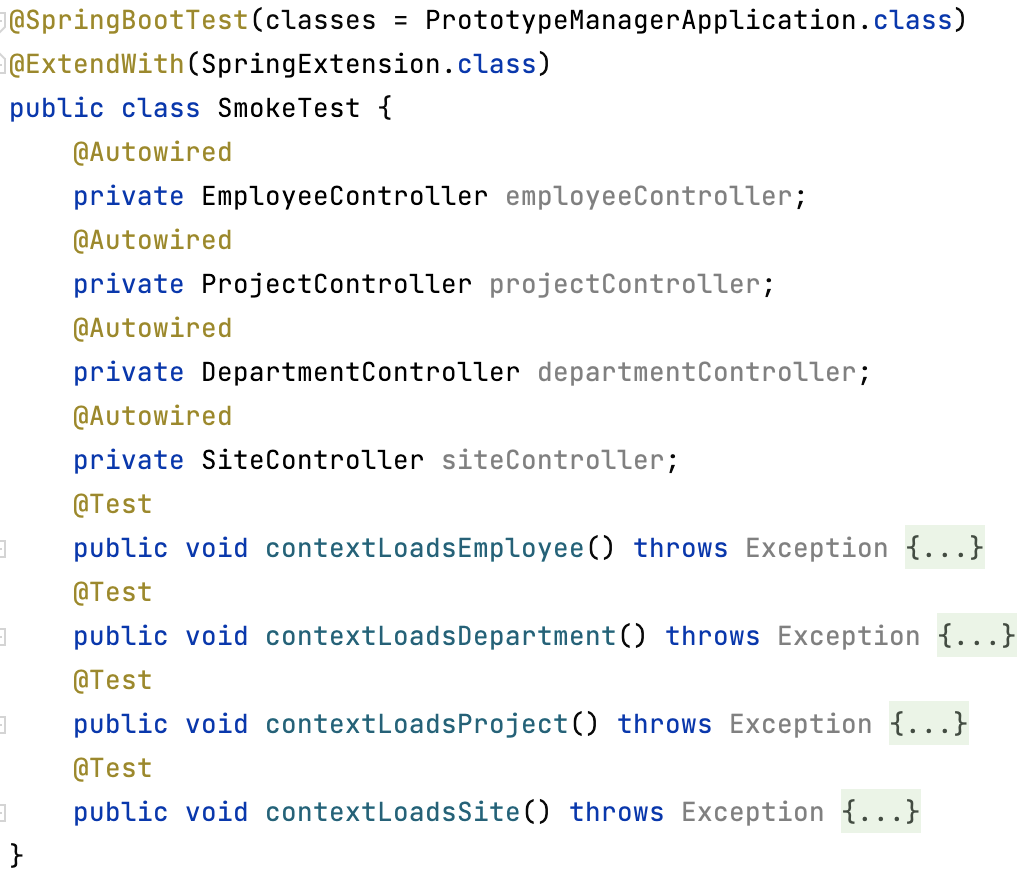
\includegraphics[width=0.7\linewidth]{immagini/SmokeTest.png}
\end{mdframed}
\caption{Classe \textit{SmokeTest} sulla creazione dei controller.}
\label{smoke-test}
\end{figure}
\FloatBarrier
Passiamo ora ai test sui metodi del controller \textit{EmployeeController}. Nell'immagine \ref{employee-controller-test} è raffigurata la classe \textit{EmployeeControllerTest} con i vari test da effettuare sul controller.
\FloatBarrier
\begin{figure}[!ht]
\begin{mdframed}
\centering
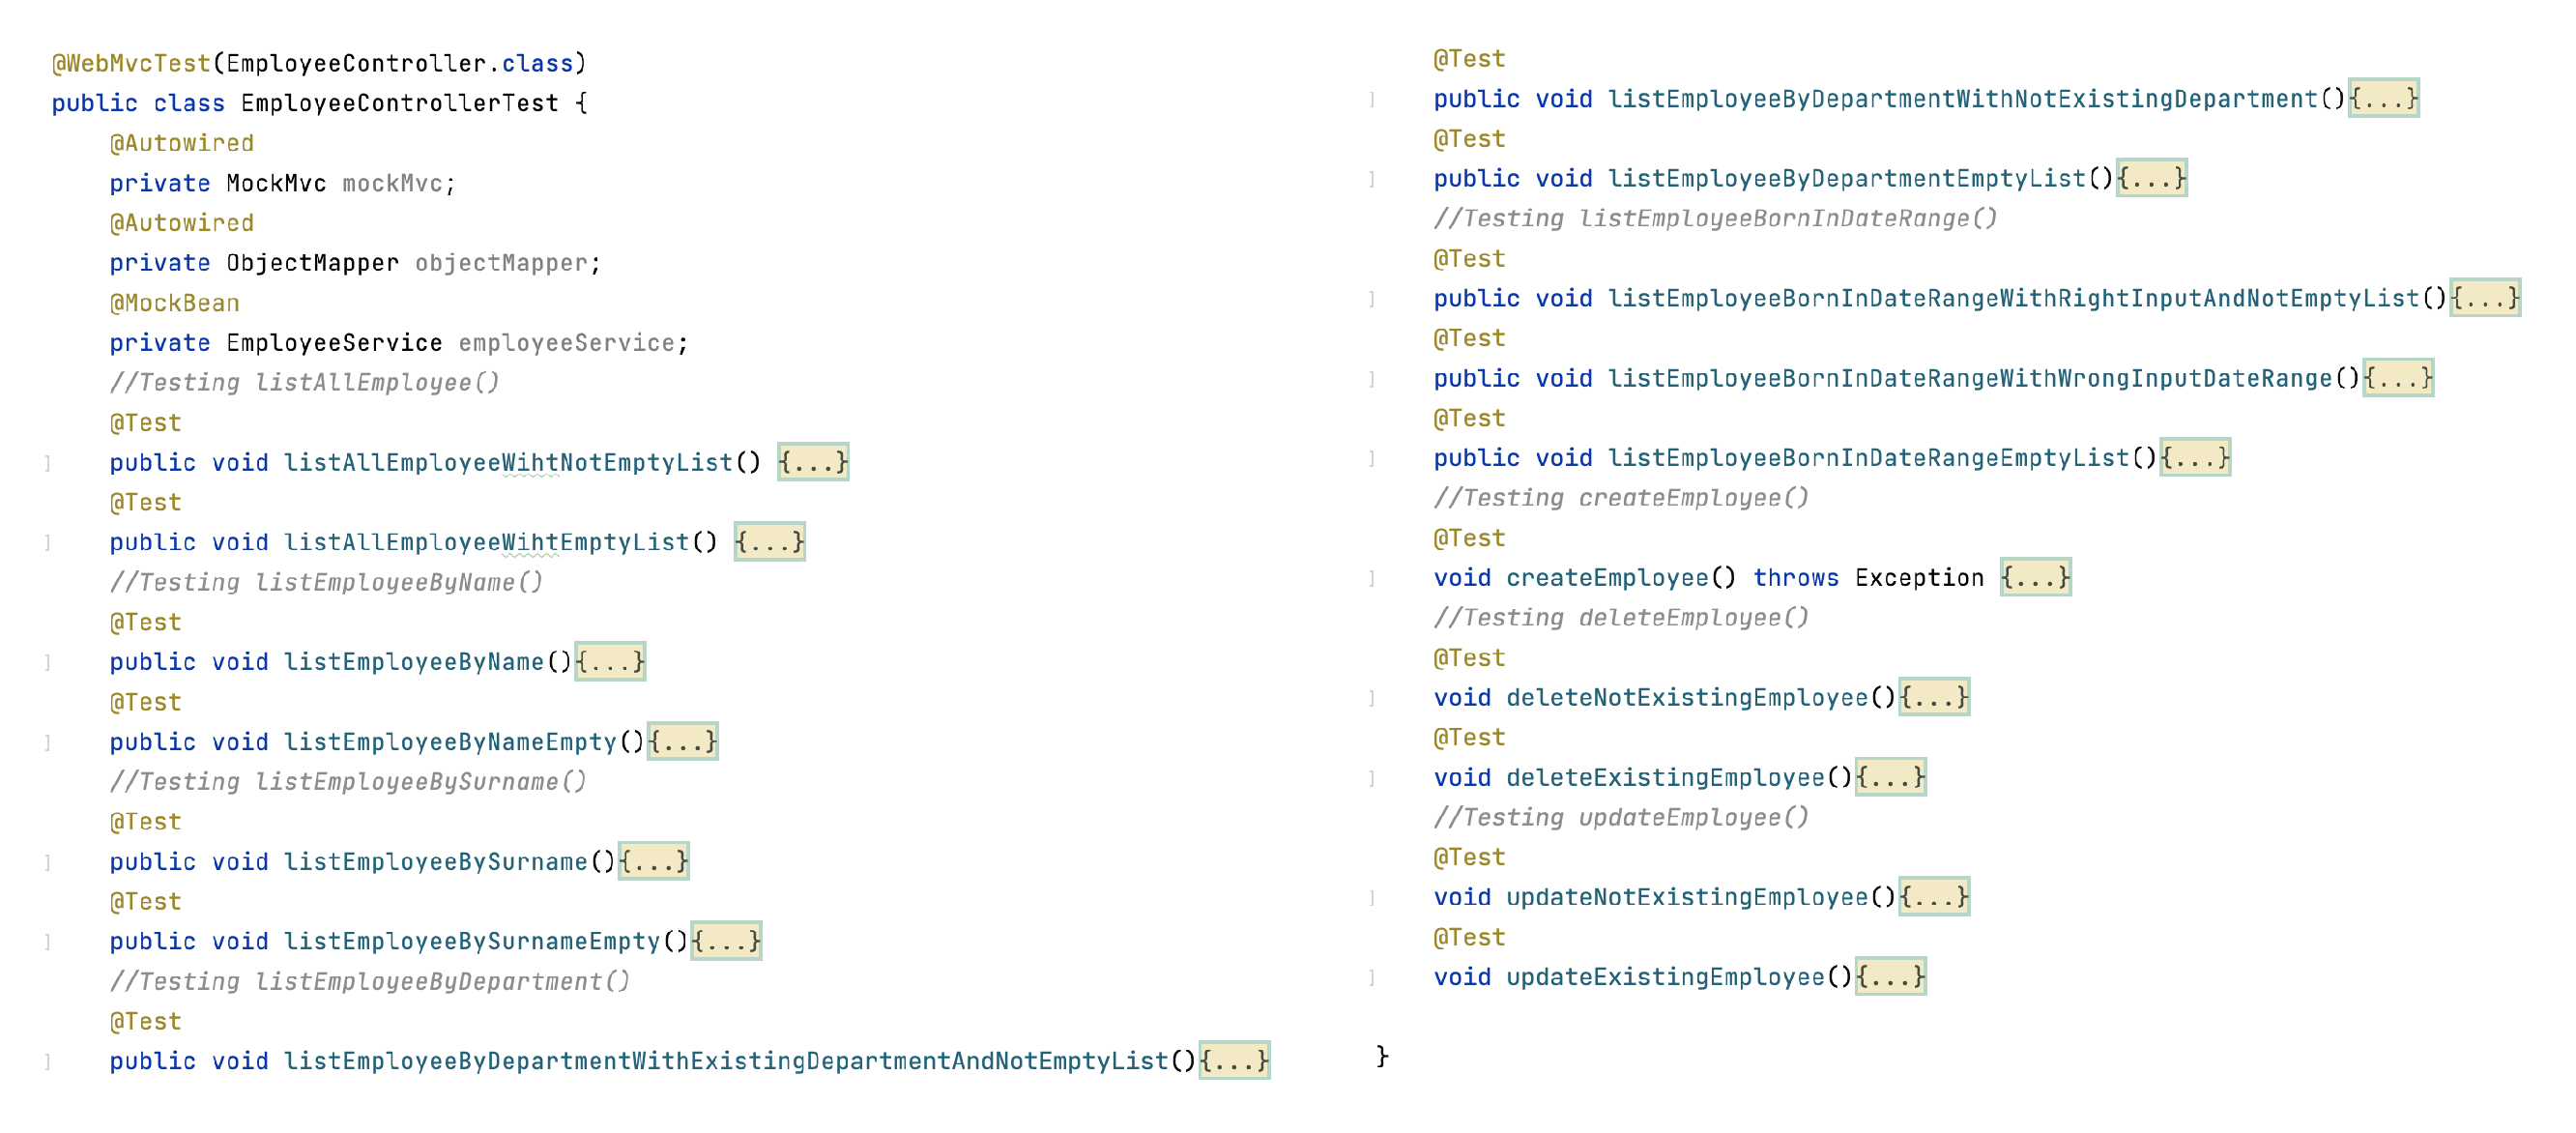
\includegraphics[width=1\linewidth]{immagini/EmployeeControllerTest.pdf}
\end{mdframed}
\caption{Classe \textit{EmployeeControllerTest}.}
\label{employee-controller-test}
\end{figure}
\FloatBarrier
La classe \textit{EmployeeControllerTest} utilizza l'annotazione \textbf{@WebMvcTest} per caricare nel contesto di test esclusivamente il controller testato.\\
Nella classe di test \textit{EmployeeControllerTest} sono dichiarate tre dipendenze fondamentali risolte con la dependency injection:
\begin{itemize}
  \item \textbf{MockMvc}: ogetto utilizzato per la simulazione di chiamate HTTP e la verifica della risposta;
  \item \textbf{ObjectMapper}: oggetto utilizzato nei test per la serializzazione e deserializzazione degli oggetti JSON in oggetti java e viceversa;
  \item \textbf{EmployeeService}: servizio che viene utilizzato nei test che usa l'annotazione \textbf{@MockBean} per aggiungere un mock dell'oggetto \textit{EmployeeService}.
\end{itemize}
Infine si riporta in figura \ref{create-employee} l'implementazione dettagliata del metodo di test \textit{createEmployee} seguendo il pattern \textit{Arrange - Act - Assert}.
\FloatBarrier
\begin{figure}[!ht]
\begin{mdframed}
\centering
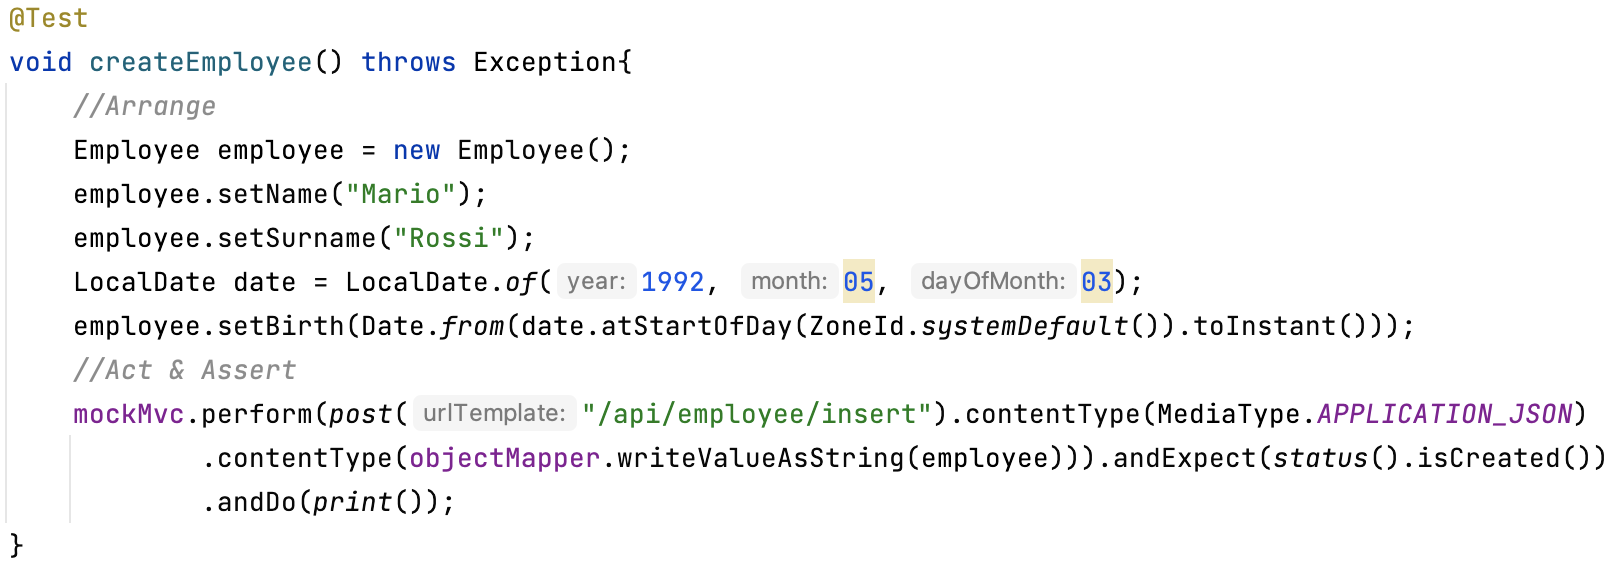
\includegraphics[width=1\linewidth]{immagini/createEmployee.png}
\end{mdframed}
\caption{Metodo di test \textit{createEmployee} della classe \textit{EmployeeControllerTest}.}
\label{create-employee}
\end{figure}
\FloatBarrier
Nella prima parte (arrange) viene creato un nuovo Employee e gli viene assegnato un nome, un cognome e una data di nascita; successivamente (act) si esegue la chiamata GET utilizzando l'oggetto \textit{MockMvc} e passando nel body della richiesta HTTP l'oggetto Java Employee trasformato in JSON grazie all'\textit{ObjectMapper}. Per ultima la fase finale (assert) in cui si verifica che lo stato di ritorno sia \textit{created}, in caso contrario il test fallisce.
\subsection{Progettazione e realizzazione frontend}
Per quanto riguarda il frontend dell'applicativo è stato utilizzato il framework Angular per realizzare una Single-Page Application. Si tratta di un frontend minimale, realizzato con il solo scopo di comprendere e sviluppare la parte di comunicazione con il server utilizzando al massimo le REST API disponibili. Per questo motivo non è stata effettuata alcuna considerazione sull'utenza e sono stati tralascati completamente aspetti quali estetica grafica, accessibilità e responsive design.\\
\subsubsection*{Architettura}
Angular segue un'architettura ben precisa, in figura \ref{angular-architecture} è possibile visualizzarne la struttura:
\FloatBarrier
\begin{figure}[!ht]
\centering
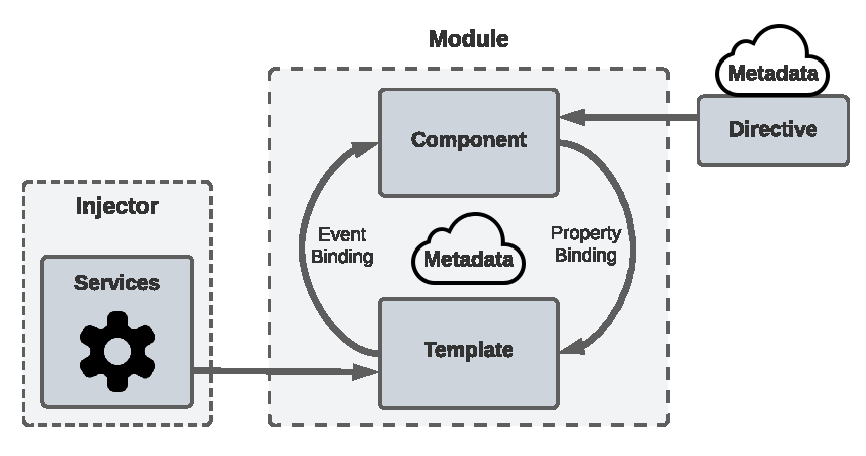
\includegraphics[width=1\linewidth]{immagini/angularArchitecture.pdf}
\caption{Architettura della Web Application del prototipo.}
\label{angular-architecture}
\end{figure}
\FloatBarrier
Si tratta di una piattaforma modulare che basa la sua struttura sulla divisione in moduli. Ciascun modulo è composto da una componente ed una viste o template; questi comunicano tra loro attraverso i metadati: l'utente che interagisce con la vista può attivare l'inizio di un procedura sulla componente. La componente spesso per l'esecuzione di alcune procedure invoca in suo aiuto i servizi iniettati nella componente stessa. \\\\
Nel corso della tesi quando si tratta il frontend verranno principalmente considerati i servizi; infatti quest'ultimi si incaricano della comunicazione con li server attraverso le API.
\subsubsection*{Funzionalità}
Di seguito si approfondisce la parte riguardante l'entità Employee, le altre entità sono state trattate in maniera analoga.\\
In linea con le query rese disponibili dal backend, devono essere presenti le seguenti funzionalità:
\begin{itemize}
  \item \textbf{Visualizzazione degli Employee}: devono poter essere visualizzata la lista degli impiegati permettendo la ricerca per: nome, cognome, data di nascita o dipartimento di appartenenza;
  \item \textbf{Aggiunta di un Employee}: deve essere possibile aggiungere un nuovo impiegato potendone specificare: nome, cognome, salario, data di nascita, dipartimento di appartenenza e infine i progetti che segue;
  \item \textbf{Aggiornamento di un Employee}: deve essere possibile aggiornare i campi dati di un impiegato specificandone l'id e il/gli campo/i da modificare;
  \item \textbf{Eliminazione di un Employee}: deve essere possibile eliminare un impiegato specificandone l'id.
\end{itemize}
Nel sezione sucessiva verrà mostrato come sono state implementate le funzionalità appena introdotte.
\subsubsection*{Realizzazione}
Inizialmente sono state create le interfacce per poter creare gli oggetti corrispondenti alle quattro entità del prototipo. Di seguito in figura \ref{employee-interface} l'esempio della dichiarazione della interfaccia dell'entità Employee:
\FloatBarrier
\begin{figure}[!ht]
\centering
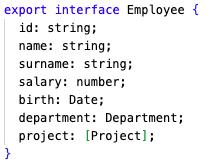
\includegraphics[width=0.3\linewidth]{immagini/employeeInterface.png}
\caption{Interfaccia di Employee.}
\label{employee-interface}
\end{figure}
\FloatBarrier
A seguire è stata implementata l'interaccia grafica inserendo nella pagina iniziale la possibilità di effettuare due scelte: la prima scelta riguarda l'entità, mentre la seconda riguarda l'operazione che si vuole eseguire sull'entità selezionata. In figura \ref{first-page} è possibile visualizzare le scelte:
\FloatBarrier
\begin{figure}[!ht]
\centering
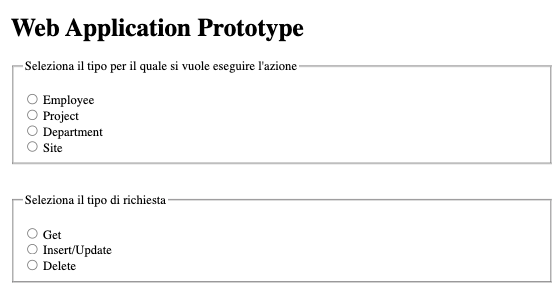
\includegraphics[width=0.7\linewidth]{immagini/firstPage.png}
\caption{Prima pagina della Web Application.}
\label{first-page}
\end{figure}
\FloatBarrier
Una volta selezionate le due opzioni viene aggiunta dinamicamente la possibilità di specificare i dettagli della richiesta. Vengono di seguito mostrate le diverse interfacce che variano al variare della scelta selezionata e il servizio che permette di eseguire la chiamata alle API del backend.\\
In figura \ref{get-employee} abbiamo il caso in cui è stata selezionata l'entità Employee con operazione GET:
\FloatBarrier
\begin{figure}[!ht]
\centering
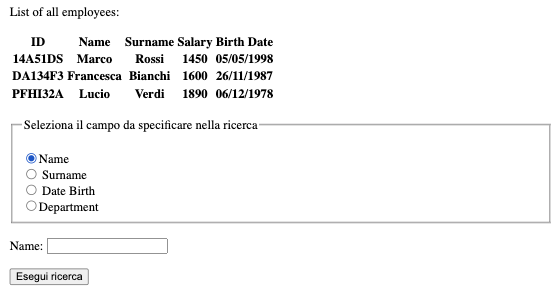
\includegraphics[width=0.7\linewidth]{immagini/getEmployee.png}
\caption{Opzioni disponibili con operazione GET selezionata.}
\label{get-employee}
\end{figure}
\FloatBarrier
Viene dunque esposta una lista contenente tutti gli impiegati, per ciascun impiegato vengono mostrati id, nome e cognome, salario e data di nascita. Successivamente viene visualizzata la scelta riguardante il campo per il quale eseguire la ricerca, in questo caso è stato scelto il nome, dunque inserendo nell'apposito campo di input il nome e selezionendo il bottone è possibile effettuare la ricerca per nome.\\
La scelta dell'opzione GET permette alla vista di invocare immediatamente il servizio che esegue una chiamata alle REST API del backend per ricevere la lista di tutti gli employee, stessa cosa accade anche quando premiamo il bottone "Esegui ricerca " dopo aver inserito il nome. Il servizio in questione si chiama \textit{EmployeeService} e di seguito in figura \ref{employee-service} ne è riportata l'implementazione:
\FloatBarrier
\begin{figure}[!ht]
\centering
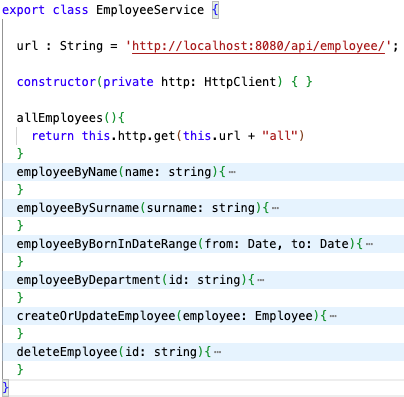
\includegraphics[width=0.6\linewidth]{immagini/employeeService.png}
\caption{Classe \textit{EmployeeService}.}
\label{employee-service}
\end{figure}
\FloatBarrier
Il servizio realizzato per le chiamate alle REST API del backend permette di essere invocato direttamente dalla componenta relativa alla vista sulla quale è stata eseguita la selezione di un elemento HTML da parte dell'utente. È inoltre presente una dipendenza con l'oggetto \textit{HttpClient}, il quale viene iniettato nel servizio venendo passato come parametro al costruttore; la sua funzionalità è quella di permettere l'esecuzione delle chiamate alle API sul backend.\\\\
Proseguendo vengono visualizzati ora i casi in cui si sceglie come operazione quella di modificare o aggiungere un nuovo impiegato. In figura \ref{post-employee} è possibile visualizzare la porzione di interfaccia grafica per l'inserimento o l'aggiornamento di un impiegato:
\FloatBarrier
\begin{figure}[!ht]
\centering
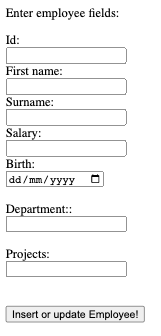
\includegraphics[width=0.3\linewidth]{immagini/postEmployee.png}
\caption{Opzioni disponibili con operazione INSERT/UPDATE selezionata.}
\label{post-employee}
\end{figure}
\FloatBarrier
Una volta inseriti tutti i valori per ciascun campo, tranne il campo ID che viene generato automaticamente, è possibile aggiungere un nuovo impiegato. Qualora invece si specificasse anche l'id, allora si tratterebbe di una modifica di un impiegato già esistente, questo solo se l'id inserito corrisponde veramente all'id di un employee. Anche in questo caso selezionando il bottone "Insert or update Employee!" viene invocato il metodo del servizio riportato in figura \ref{employee-service}.\\
Per finire in figura \ref{delete-employee} il caso in cui venga selezionata l'opzione DELETE:
\FloatBarrier
\begin{figure}[!ht]
\centering
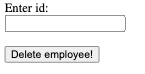
\includegraphics[width=0.3\linewidth]{immagini/deleteEmployee.png}
\caption{Opzioni disponibili con operazione DELETE selezionata.}
\label{delete-employee}
\end{figure}
\FloatBarrier
\subsubsection*{Testing}
I test di unità sono stati implementati seguendo il pattern \textit{Arrange - Act - Assert} sui metodi del servizio riportato in figura \ref{employee-service}. Di seguito nell'immagine \ref{employee-service-tests} è possibile visualizzare la funzione \textit{describe} la quale viene utilizzata per raggruppare un insieme di test:
\FloatBarrier
\begin{figure}[!ht]
\centering
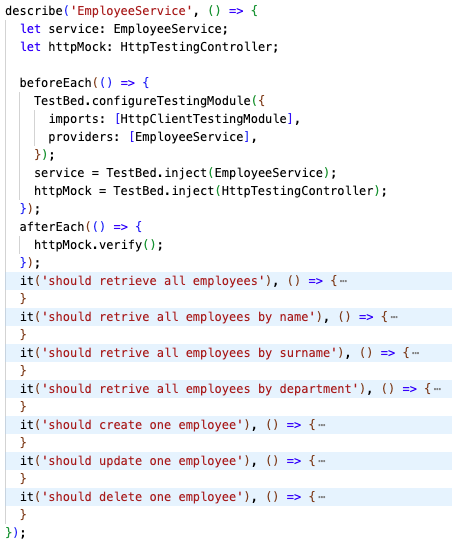
\includegraphics[width=0.6\linewidth]{immagini/employeeServiceTest.png}
\caption{Test per i metodi del servizio \textit{EmployeeService}.}
\label{employee-service-tests}
\end{figure}
\FloatBarrier
Viene incluso il modulo Angular \textit{HttpClientTestModule}, necessario al fine di importare il servizio iniettabile \textit{HttpTestingController} utilizzato per il mocking e il flushing e dunque per eliminare le microtask in sospeso. Sono inoltre presenti le funzioni \textit{BeforeEach} utilizzata per configurare l'ambiente di test, dunque importare i moduli necessari e risolvere le dipendenze e la funzione \textit{afterEach} utilizzata per controllare, dopo l'esecuzion di ciascun test, che non siano rimaste richieste in sospeso. Infine, con la funzione \textit{it} viene definito un titolo per ciascun test e implementato il test stesso.\\
Più nello specifico in figura \ref{get-all-test} si può visualizzare l'implementazione di un test per il metodo \textit{allEmployee} del servizio \textit{EmployeeService}:
\FloatBarrier
\begin{figure}[!ht]
\centering
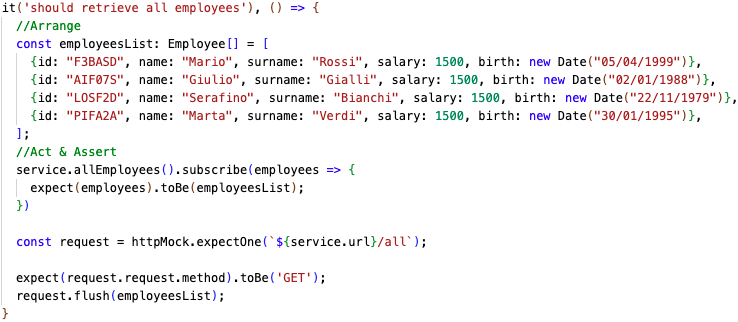
\includegraphics[width=0.8\linewidth]{immagini/allEmployeeTest.png}
\caption{Test sul metodo \textit{allEmployee()} di \textit{EmployeeService}.}
\label{get-all-test}
\end{figure}
\FloatBarrier
Viene inizialmente creato un array di Employee che ci si aspetterà di ricevere dalla chiamata e sucessivamente si verifica il risultato atteso tramite la funzione \textit{expect}.Per finire si controlla che l'url sia corretto, che venga effettuata una sola chiamata GET e che si tratti effettivamente di una richiesta GET.
\subsection{Migrazione da REST a GraphQL}
In questa sezione si affronta la migrazione sia del backend che del frontend da REST API a GraphQL API.
\subsubsection*{Migrazione Backend}
Il backend realizzato in Spring Boot con l'aiuto del modulo Spring Data REST per la realizzazione dei controller di REST API deve essere riscritto in parte utilizzando il modulo Spring GraphQL per la realizzazione dei controller in GraphQL.\\
É stata adottata la tecnica \textit{Schema First} che prevede la costruzione del GraphQL Schema ed, a seguire, l'implementazione dei resolver delle API. Nonostante i resolver fossero già realizzati per il prototipo in REST è comunque necessario adattarli all'utilizzo di questo nuovo protocollo.\\
Le quattro entità presenti, ovvero Employee, Project, Department e Site devono essere riportate tutte nel GraphQL schema poiché sono tutte accessibili dal client; esse saranno definite sia come entità di input che di output poiché GraphQL differenzia i due tipi nelle query, mutation e subscription. In figura \ref{employee-schema} è possibile visualizzare l'implementazione dei tipi \textit{Employee} e \textit{EmployeeInput}.
\FloatBarrier
\begin{figure}[!ht]
\centering
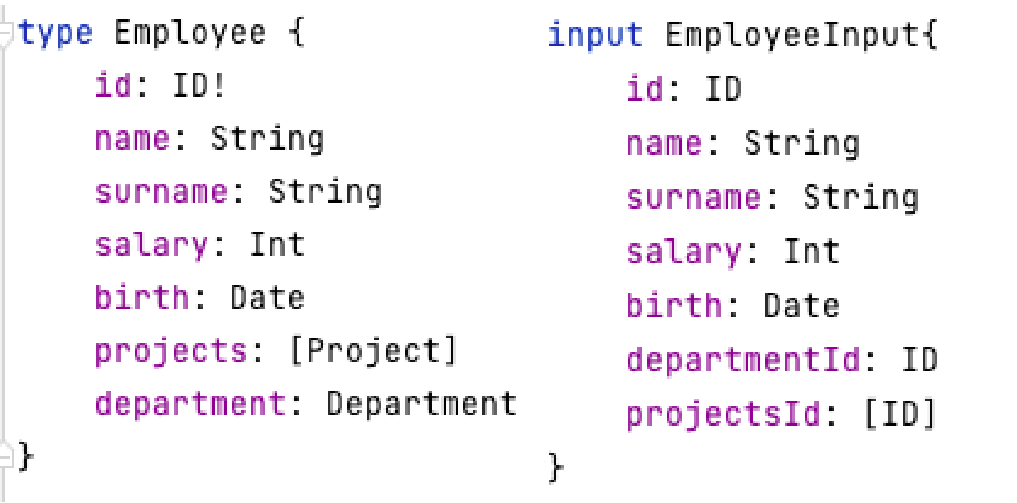
\includegraphics[width=0.8\linewidth]{immagini/employeeSchema.pdf}
\caption{Tipi \textit{Employee} e \textit{EmployeeInput} nel GraphQL Schema.}
\label{employee-schema}
\end{figure}
\FloatBarrier
Come si può notare i due tipi \textit{Employee} e \textit{EmployeeInput} non corrispondono completamente: i campi \textit{projects} e \textit{department} di \textit{Employee} non sono presenti in \textit{EmployeeInput}, o  meglio sono presenti ma in diversa forma. Il motivo di tale differenza si può sintetizzare in questo modo:
\begin{itemize}
  \item il tipo \textit{Employee} verrà ritornato al client su richiesta; dovrà contenere le varie istanze dei progetti a cui un impiegato sta partecipando come pure l'oggetto dipartimento;
  \item il tipo \textit{EmployeeInput} indica come fornire i dati necessari all'aggiunta/aggiornamento dell'impiegato; è sufficiente dunque passare gli id dei progetti coinvolti come pure l'id del dipartimento dell'impiegato.
\end{itemize}
A questo punto è possibile definire le query, le mutation ed eventualmente le subscription che si vogliono rendere disponibili al client. In figura \ref{query-employee} è possibile visualizzare la dichiarazione delle query, mutation e della subscription riguardanti l'entità Employee.
\FloatBarrier
\begin{figure}[!ht]
\centering
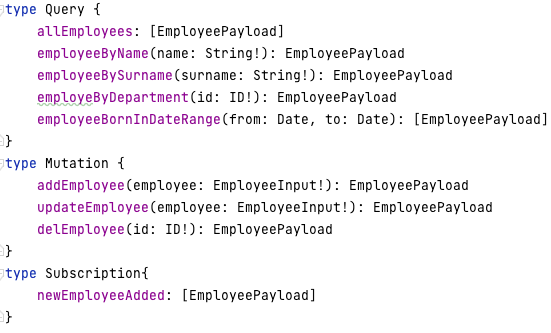
\includegraphics[width=0.6\linewidth]{immagini/queryEmployee.png}
\caption{Implementazione delle query, mutation e subscription nel GraphQL Schema.}
\label{query-employee}
\end{figure}
\FloatBarrier
Il dato ritornato è di tipo \textit{Employee} per tutte le operazioni mentre quello di input è \textit{EmployeeInput}.\\
È stata aggiunta inoltre una subscription per sfruttare a pieno le funzionalità di GraphQL. Questa subscription permette al client di ricevere i nuovi impiegati aggiunti senza per forza richiederli.
\paragraph{Migrazione dei controller}
La migrazione non coinvolge gli strati di servizio e repository in quanto non è necessario apportare modifiche alle logiche e alla gestione del database. L'unico strato da riscrivere parzialmente è lo strato del controller.\\
Come prima cosa si realizzano le classi Java corrispondenti ai tipi di input; questo è necessario poiché nei metodi del controller è previsto come parametro di input la versione di input dell'impiegato.\\
L'implementazione del controller risulta differente rispetto a quella vista con le REST API. Di seguito in figura \ref{graphql-controller} è possibile visualizzarne la struttura ed i metodi:
\FloatBarrier
\begin{figure}[!ht]
\centering
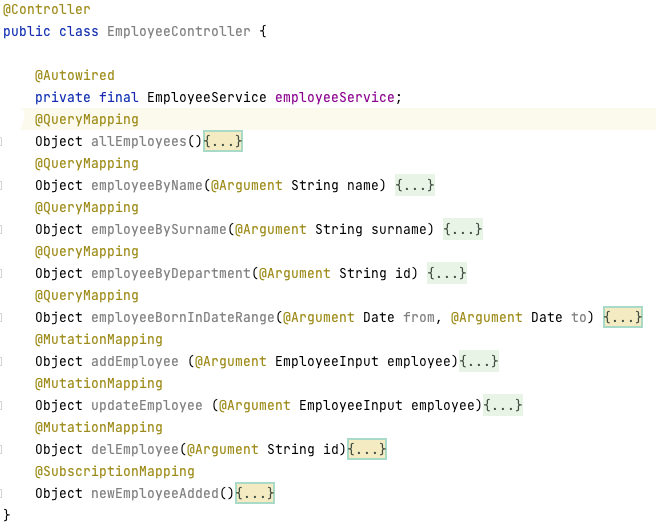
\includegraphics[width=0.8\linewidth]{immagini/graphQLEmployeeController.png}
\caption{Classe \textit{EmployeeController}.}
\label{graphql-controller}
\end{figure}
\FloatBarrier
Come si può notare si tratta di un controller simile a quello REST nei metodi, tuttavia le annotazioni e alcune implementazioni differiscono. Vengono utilizzate le annotazioni:
\begin{itemize}
  \item \textbf{@Controller}: indica che si tratta di un generico controller (non più REST controller);
  \item \textbf{@QueryMapping}: attribuito ai metodi che risolvono le query;
  \item \textbf{@MutationMapping}: attribuito ai metodi che risolvono le mutation;
  \item \textbf{@SubscriptioMapping}: attribuito al metodo che risolve la subscription;
  \item \textbf{@Argument}: utilizzato per specificare gli argomenti.
\end{itemize}
Queste annotazioni sono fondamentali poiché permettono di effettuare il mapping tra i tipi, le query, le mutation e le subscription definiti nel GraphQL Schema e quelli definiti nel controller. Per questo motivo il nome di ciascun metodo o tipo negli argomenti deve corrispondere esattamente al nome nel GraphQL Schema, altrimenti il mapping non andrà a buon fine e verranno generati degli errori.\\
L'implementazione dei metodi del controller risulta simile a quella dei corrispettivi metodi nel REST controller. Tuttavia, trattandosi di una particolare funzionalità disponibile esclusivamente in GraphQL, in figura \ref{subscription-graphql} viene riportata l'implementazione della subscription \textit{newEmployeeAdded}:
\FloatBarrier
\begin{figure}[!ht]
\centering
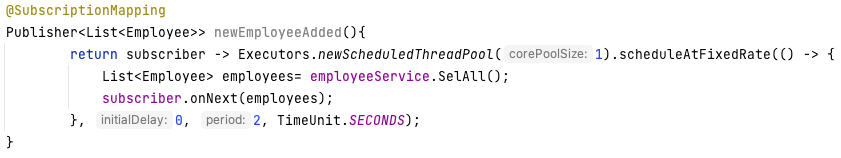
\includegraphics[width=1\linewidth]{immagini/newEmployeeAdded.png}
\caption{Subscription \textit{newEmployeeAdded}.}
\label{subscription-graphql}
\end{figure}
\FloatBarrier
L'implementazione della subscription permette al subscriber, in questo caso il client, di ricevere la lista aggiornata al verificarsi di un evento. L'oggetto \textit{Publisher<>} permette di inviare la lista aggiornata a tutti i subscribers in tempo reale, così facendo il client non dovrà richiedere periodicamente la lista con la query \textit{allEmployee}.
\textcolor{red}{Mancano test in graphQL}
\paragraph{Strutture delle risposte HTTP in GraphQL e gestione degli errori}
Le risposte che il server GraphQL ritorna al client in seguito ad una query, mutation o subscription sono dei file JSON. Questi JSON possono contenere tre tipi di campi:
\begin{itemize}
  \item \textbf{Data}: ritornato nella risposta solo in caso di successo, assume valore \textit{null} al presentarsi di un errore;
  \item \textbf{Errors}: ritornato solo ed esclusivamente al verificarsi di uno o più errori, contiene le informazioni necessarie all'interpretazione dell'anomalia;
  \item \textbf{Extensions}: campo facoltativo a disposizione degli sviluppatori di backend, può essere utilizzato ad esempio per ritornare il timestamp dell'esecuzione della query.
\end{itemize}
Analizzando gli errori che si possono verificare durante l'esecuzione di una query, mutation o subscription nel server GraphQL, si individuano tre categorie:
\begin{itemize}
  \item \textbf{Errori di sintassi}: si tratta di errori nella sintassi della query. Se la query è sintatticamente scorretta l'errore sarà di tipo "Syntax Error"; in questo caso l'esecuzione della query non parte nemmeno;
  \item \textbf{Errori di validazione}: si verificano quando vengono specificati nella richiesta tipi non coerenti con lo schema. In questo caso l'errore si verifica durante l'esecuzione, dunque viene ritornato sia il campo \textit{data}, con valore null o con i dati parziali che il server è riuscito a recuperare, che il campo \textit{errors} che indica la presenza di uno o più errori di data fetching;
  \item \textbf{Errori nei resolver:} si verificano durante la risoluzione della query e non sono legati al fatto che la query sia formulata male o con tipi sbagliati. Questi errori devono essere gestiti lato server;
\end{itemize}
Quando si verificano errori di sintassi o validazione la risposta l'errore ritornato indica perfettamente la natura dell'errore. La terza tipologia di errore quasi sempre risulta incomprensibile dal client. Questo accade perché la gestione delle eccezioni durante l'esecuzione di una richiesta è presa in carico dall'interfaccia predefinita \textit{DataFetcherExceptionHandler} la quale permette la dichiarazione di più risolutori di eccezioni detti \textit{DataFetcherExceptionResolver}. Questi ultimi vengono invocati sequenzialmente fino a quando uno di essi è in grado di risolvere l'eccezione; in caso contrario viene ritornata una informazione di errore incomprensibile con categoria \textit{"INTERNAL\_ERROR"}. Questo per uno sviluppatore può essere un problema poiché non è facile individuare la provenienza dell'errore. Per questo motivo sono stati creati differenti resolvers per le varie eccezioni che possono verificarsi. In figura \ref{resolver-example} l'esempio di implementazione di un resolver che riscrive il metodo di risoluzione delle eccezioni \textit{resolveToSingleError} al fine di risolvere l'eccezione \textit{EmployeeNotFound}.
\FloatBarrier
\begin{figure}[!ht]
\centering
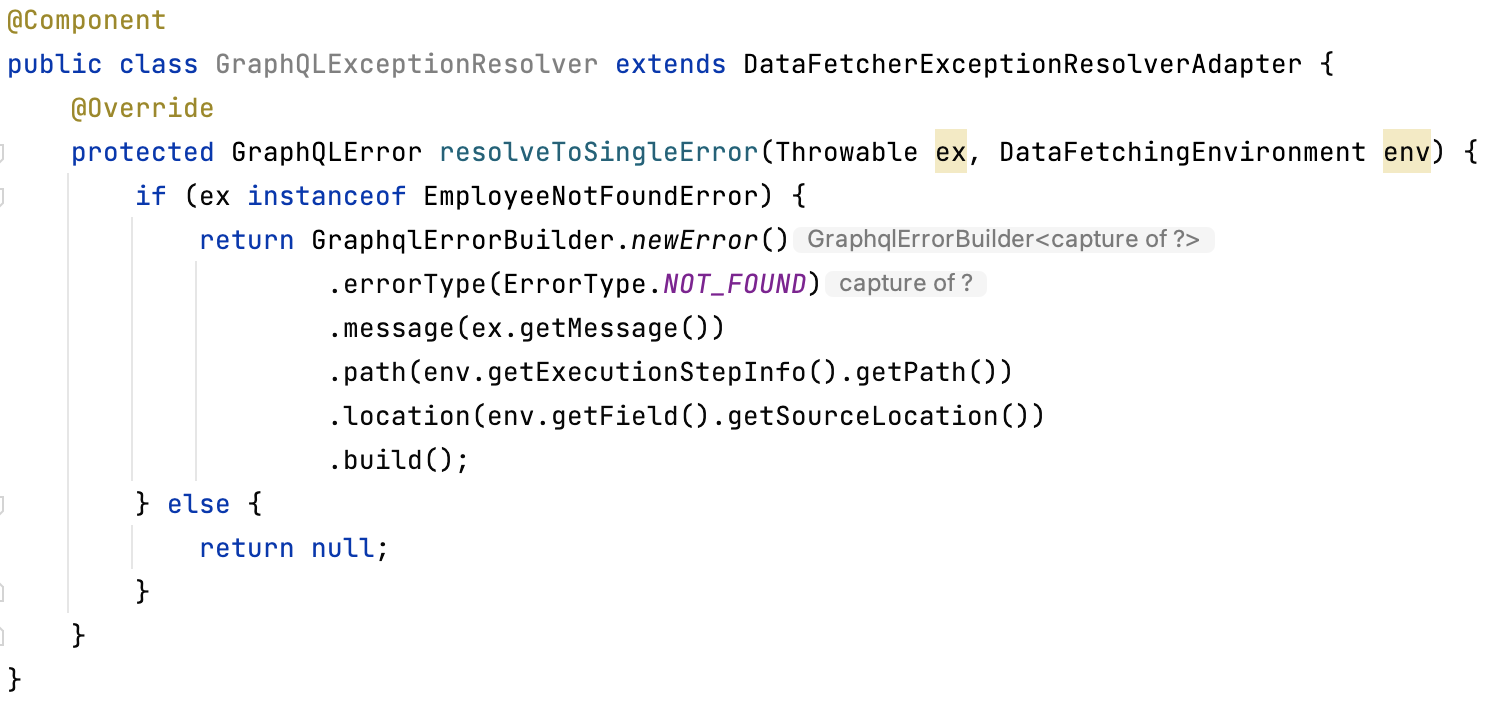
\includegraphics[width=0.8\linewidth]{immagini/resolverExample.png}
\caption{Classe \textit{GraphQLExceptionResolver} con metodo \textit{resolveToSingleError} ridefinito per la risoluzione dell'eccezione \textit{EmployeeNotFoundError}.}
\label{resolver-example}
\end{figure}
\FloatBarrier
Com'è possibile notare viene ritornato un oggetto di tipo \textit{GraphQLError} con i campi impostati correttamente. Al presentarsi dell'eccezione il client sarà ora in grado di comprendere il motivo di errore.
\subsubsection*{Migrazione Frontend}
La migrazione del frontend richiede uno sforzo minore rispetto al backend, infatti è sufficiente effettuare la migrazione esclusivamente dei servizi che si occupano dell'invocazione delle API.\\
Il servizio visualizzato precedentemente in figura \ref{employee-service} \textit{EmployeeService} non cambia la sua struttura; i metodi rimangono gli stessi, tuttavia l'implementazione del metodo deve cambiare. Oltre all'implementazione dei metodi cambia anche l'oggetto che permette il fetching dei dati dal server, infatti trattandosi ora di un GraphQL Server, sarà necessaria la dipendenza dall'oggetto \textit{Apollo} utilizzato nel fetching dei dati da un server GraphQL.\\
In figura \ref{employee-service-method-graphql} è possibile visualizzare l'implementazione del metodo  \textit{allEmployees}.
\FloatBarrier
\begin{figure}[!ht]
\centering
\includegraphics[width=0.5\linewidth]{immagini/employeeServiceMethodGraphql.png}
\caption{Metodo \textit{allEmployees()} della classe  \textit{EmployeeService}.}
\label{employee-service-method-graphql}
\end{figure}
\FloatBarrier
Attraverso il metodo \textit{watchQuery<>} dell'oggetto \textit{apollo} è possibile eseguire la query all'endopoint del server GraphQL. Il metodo ritorna un oggetto di tipo \textit{Observable} ed il subscriber dovrà occuparsi di gestire quanto ritornato dal servizio. Nel caso in cui la query sia andata a buon fine dovrà leggere le informazioni presenti nel campo \textit{"data"}; nel caso contrario dovrà occuparsi di mostrare il messaggio ed il tipo dell'errore presente nel campo \textit{"errors"}.
\section{SushiLab}
\label{sushi-lab}
\subsection{Confronto con stakeholder}
Circa dopo un mese dall'inizio dello stage è stato realizzato un confronto con gli stakeholder. Con il tutor interno dell'azienda SyncLab, ovvero Fabio Pallaro sono stati valutati alcuni applicativi già implementati che seguissero l'architettura server - client per effettuarne la migrazione da REST API a GraphQL API.\\
Tra tutti l'applicativo selezionato è stato \textbf{SushiLab}, il quale è stato realizzato da alcuni stagisti nei mesi precedenti. Il motivo che ci ha portato a concordare questa scelta è stato principalmente il fatto che fosse un applicativo con una struttura API sviluppata.
\subsection{Comprensione dell'applicativo e obbiettivi}
SushiLab è un applicativo che mira ad automatizzare il processo di tracciamento degli ordini nei ristoranti di sushi all you can eat. Si tratta da un applicativo composto da:
\begin{itemize}
  \item \textbf{Backend}: realizzato un backend in Java con il framework Spring Boot, gestisce un inoltre database PostgreSQL;
  \item \textbf{Frontend}: realizzato in Typescript con il framework Angular;
  \item \textbf{Componente di Machine Learning}: utilizzata per il riconoscimento dei piatti tramite la fotocamera del telefono;
  \item \textbf{Applicativo mobile}: la versione mobile della web app sotto forma di applicazione.
\end{itemize}
Il mio intervento sull'applicativo prevede di lavorare sulla comunicazione tra backend e frontend, effettuando una migrazione completa delle REST API sviluppate portandole a GraphQL API, esattamente come è stato fatto per il prototipo.\\\\
Di seguito nelle sottosezioni verranno analizzate le strutture del backend e del frontend, tralasciando gli aspetti implementativi specifici già visualizzati per il prototipo e concentrandosi principalmente sulla parte di comunicazione tramite API.
\subsection{Panoramica del backend}
Il backend sviluppato in Java con il framework Spring Boot segue l'architettura proposta per il prototipo, ovvero il pattern repository - service - controller. Di seguito verranno analizzate e descritte brevemente le componenti principali degli strati di persistenza e di business logic, mentre verrà approfondito lo strato di controller.
\subsubsection{Entità}
In figura \ref{ER-sushilab} è possibile visualizzare lo schema ER delle entità presenti e le relazioni che intercorrono. Vengono tralasciati i campi per non entrare eccessivamente nel dettaglio.
\FloatBarrier
\begin{figure}[!ht]
\centering
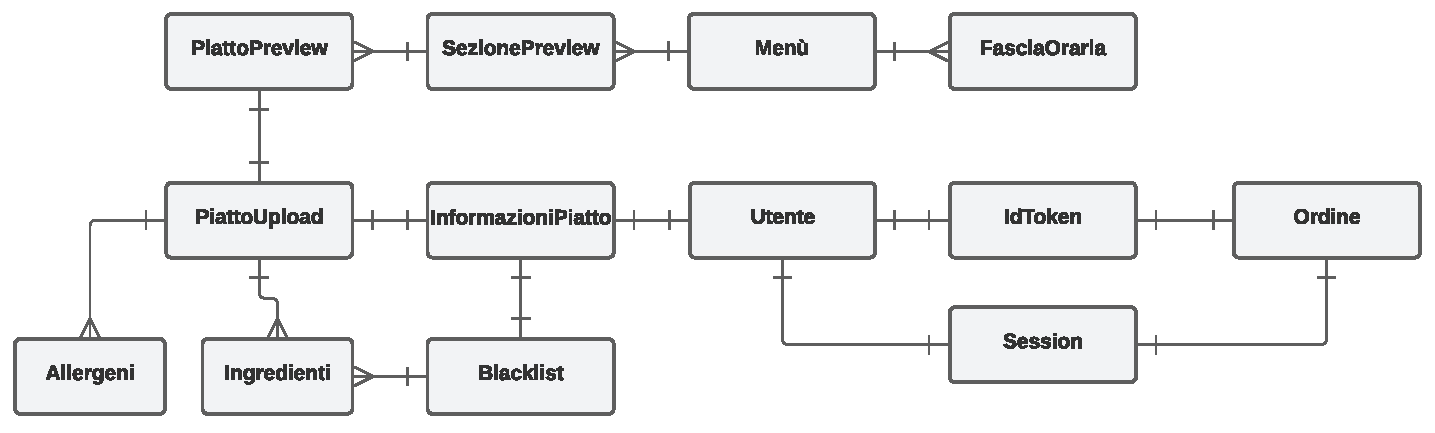
\includegraphics[width=1\linewidth]{immagini/ER_sushilab.pdf}
\caption{Diagramma ER di \textit{SushiLab}.}
\label{ER-sushilab}
\end{figure}
\FloatBarrier
Sono dunque presenti le entità:
\begin{itemize}
  \item \textbf{PiattoUpload}: una tipo di piatto con allergeni e ingredienti;
  \item \textbf{PiattoPreview}: l'anteprima di piatto associata ad un \textit{PiattoUpload};
  \item \textbf{SezionePreview}: un insieme di piatti di una particolare categoria;
  \item \textbf{Menù}: un insieme di sezioni di piatti, si tratta del menù di un ristorante;
  \item \textbf{Utente}: l'utente registrato, può anche essere un gestore e dunque essere il proprietario del ristorante e dunque poter apportare delle modifiche ai menù, ai piatti, ecc..;
  \item \textbf{FasciaOraria}: una fascia oraria in cui può essere disponibile un Menù;
  \item \textbf{InformazioniPiatto}: le caratteristiche di un singolo utente riguardo ingredienti che non può mangiare, se gli è piaciuto un piatto specifico o se ha preferenze per particolari tipi di menù;
  \item \textbf{Blacklist}: l'insieme di ingredienti che un cliente preferisce non mangiare;
  \item \textbf{IdToken}: un token identificativo associato ad un utente quando partecipa ad un tavolo;
  \item \textbf{Session}: la situazione di un singolo tavolo in un determinato momento con determinati clienti, quando un cliente si siede ad un tavolo può aprire una sessione e invitare gli amici allo stesso tavolo;
  \item \textbf{Ordine}: gli ordini effettuati in una specifica sessione o da una specifica persona;
  \item \textbf{Allergeni}: le sostanze che tipicamente possono causare allergie;
  \item \textbf{Ingredienti}: i possibili ingredienti nei vari piatti;
\end{itemize}
Ciascuna di queste entità ha la corrispettiva classe Java nel backend. Per ciascuna entità è stata realizzata la corrispettiva repository estendendo l'interfaccia \textit{JPARepository<T, ID>} per la gestione dei dati e delle risorse nel database.
\subsubsection*{Servizi}
Lo strato di servizio presente prevede la definizione di solo due classi per la gestione delle logiche del backend. Di seguito vengono elencate le funzioni dei due servizi.
\paragraph{ClientService}
Il primo servizio gestisce le logiche delle possibili richieste del client. Questo servizio permette la gestione di:
\begin{itemize}
  \item \textbf{Utenti}: permette tutte le operazioni di login, registrazione di un nuovo utente, aggiunta dell'IdToken ad un utente all'apertura di una nuova sessione ad un tavolo e infine il recupero e modifica della password;
  \item \textbf{Preferenze Utente}: permette di modificare le preferenze di un utente e modificare, aggiungere o eliminare le valutazioni attribuite ai piatti; inoltre permette di visualizzare gli ingredienti nella blacklist di uno specifico utente;
  \item \textbf{Sessioni}: permette di craere ed eliminare le sessioni;
  \item \textbf{Ordini}: permette la gestione degli ordini da parte di un utente, di aggiungerne di nuovi o di visualizzarli;
  \item \textbf{Gestore}: permette di verificare che un utente corrispondi o meno al gestore;
  \item \textbf{Menu}: permette di visualizzare il menù di un ristorante.
\end{itemize}
\paragraph{GestoreService}
Il servizio \textit{GestoreService} gestisce le logiche riguardanti le operazioni realizzabili da un utente gestore, dunque permette:
\begin{itemize}
  \item \textbf{Piatti}: la gestione dei piatti, è possibile visualizzarli, eliminarli, modificarli e aggiungerne di nuovi;
  \item \textbf{Menu}: la gestione del menù, è possibile riorganizzarlo diversamente e attribuirgli differenti fasce orarie di disponibilità.
\end{itemize}
\subsubsection*{Controller}
Infine abbiamo lo strato più importante per gli scopi della tesi. Si tratta dello strato di controller il quale prevede cinque controller principali, di seguito verranno analizzati tutti i metodi di ciascun controller tralasciandone gli aspetti implementativi.
\paragraph{LoginController}
Il seguente controller dichiara una dipendenza con il servizio \textit{ClientService}. Di seguito la tabella dei metodi:
%//////////////////////// INIZIO TABELLA ////////////////////////
%//////////////////////// INIZIO TABELLA ////////////////////////
\begin{table}[!h]
\renewcommand{\arraystretch}{1.1}
\centering
\begin{tabular}{|c|c|c|l|}
\hline
\rowcolor[HTML]{C0C0C0}
{\color[HTML]{000000} \textbf{Metodo}} & {\color[HTML]{000000} \textbf{Parametri}} & {\color[HTML]{000000} \textbf{Descrizione}}                                           & {\color[HTML]{000000} \textbf{Azione}} \\ \hline
\textbf{eseguiLogin}                   & Utente utente             & \begin{tabular}[c]{@{}c@{}}Controlla ed effettua\\ il login di un utente\end{tabular} & POST                           \\ \hline
\end{tabular}
\caption{Metodi del controller \textit{LoginController}.}
\end{table}
%//////////////////////// FINE TABELLA ////////////////////////
%//////////////////////// FINE TABELLA ////////////////////////
\paragraph{UtenteController}
Questo controller dichiara una dipendenza con il servizio \textit{ClientService} ed è composto dai metodi nella specificati nella seguente tabella:
%//////////////////////// INIZIO TABELLA ////////////////////////
%//////////////////////// INIZIO TABELLA ////////////////////////
\begin{table}[!h]
\renewcommand{\arraystretch}{1.2}
\begin{tabular}{|c|c|c|c|}
\hline
\rowcolor[HTML]{C0C0C0}
{\color[HTML]{000000} \textbf{Metodo}}        & {\color[HTML]{000000} \textbf{Parametri}}                                                                              & {\color[HTML]{000000} \textbf{Descrizione}}                                                                                                                & {\color[HTML]{000000} \textbf{Azione}} \\ \hline
{\color[HTML]{000000} \textbf{ottieniUtente}}          & {\color[HTML]{000000} String idPersona}                                                                                & {\color[HTML]{000000} \begin{tabular}[c]{@{}c@{}}Ricerca un utente\\ per id\end{tabular}}                                                                  & {\color[HTML]{000000} GET}             \\ \hline
\rowcolor[HTML]{EFEFEF}
{\color[HTML]{000000} \textbf{registraUtente}}         & {\color[HTML]{000000} Utente utente}                                                                                   & {\color[HTML]{000000} \begin{tabular}[c]{@{}c@{}}Aggiunge un nuovo\\ utente\end{tabular}}                                                                  & {\color[HTML]{000000} POST}            \\ \hline
{\color[HTML]{000000} \textbf{modificaStatoPreferiti}} & {\color[HTML]{000000} \begin{tabular}[c]{@{}c@{}}String idPersona\\ String idPiatto\end{tabular}}                   & {\color[HTML]{000000} \begin{tabular}[c]{@{}c@{}}Modifica i preferiti\\ di un utente,  con gli \\ dei piatti\end{tabular}}                                 & {\color[HTML]{000000} POST}            \\ \hline
\rowcolor[HTML]{EFEFEF}
{\color[HTML]{000000} \textbf{modificaValutazione}}    & {\color[HTML]{000000} \begin{tabular}[c]{@{}c@{}}String idPersona\\ String idPiatto\\ String param\end{tabular}} & {\color[HTML]{000000} \begin{tabular}[c]{@{}c@{}}Modifica la \\ valutazione di una \\ persona rispetto ad \\ un piatto con nuovi\\ parametri\end{tabular}} & {\color[HTML]{000000} POST}            \\ \hline
{\color[HTML]{000000} \textbf{recuperoPassword}}       & {\color[HTML]{000000} String param}                                                                                    & {\color[HTML]{000000} \begin{tabular}[c]{@{}c@{}}Ritorna la password\\ recuperata se vengono\\ forniti i parametri\\ necessari\end{tabular}}               & {\color[HTML]{000000} POST}            \\ \hline
\rowcolor[HTML]{EFEFEF}
{\color[HTML]{000000} \textbf{verificaCodice}}         & {\color[HTML]{000000} String param}                                                                                    & {\color[HTML]{000000} \begin{tabular}[c]{@{}c@{}}Verifica il codice\\ di recupero password\end{tabular}}                                                   & {\color[HTML]{000000} POST}            \\ \hline
{\color[HTML]{000000} \textbf{reimpostaPassword}}      & {\color[HTML]{000000} String param}                                                                                    & {\color[HTML]{000000} \begin{tabular}[c]{@{}c@{}}Imposta una nuova \\ password per un utente\end{tabular}}                                                 & {\color[HTML]{000000} POST}            \\ \hline
\rowcolor[HTML]{EFEFEF}
{\color[HTML]{000000} \textbf{aggiornaBlacklist}}      & {\color[HTML]{000000} \begin{tabular}[c]{@{}c@{}}String idPersona\\ Ingredienti ingredienti\end{tabular}}           & {\color[HTML]{000000} \begin{tabular}[c]{@{}c@{}}Aggiorna la blacklist \\ di una persona con i \\ nuovi ingredienti\end{tabular}}                          & {\color[HTML]{000000} POST}            \\ \hline
{\color[HTML]{000000} \textbf{ottieniBlacklist}}       & {\color[HTML]{000000} String idPersona}                                                                                & {\color[HTML]{000000} \begin{tabular}[c]{@{}c@{}}Ritorna la lista di \\ ingredienti nella \\ blacklist di un utente\end{tabular}}                          & {\color[HTML]{000000} GET}             \\ \hline
\end{tabular}
\caption{Metodi del controller \textit{UtenteController}.}
\end{table}
%//////////////////////// FINE TABELLA ////////////////////////
%//////////////////////// FINE TABELLA ////////////////////////
\paragraph{TavoloController}
Anche il seguente controller dichiara una dipendenza con \textit{ClientService} e i suoi metodi gestiscono gli utenti, gli ordini ed i tavoli.
% Please add the following required packages to your document preamble:
% \usepackage[table,xcdraw]{xcolor}
% If you use beamer only pass "xcolor=table" option, i.e. \documentclass[xcolor=table]{beamer}
% Please add the following required packages to your document preamble:
% \usepackage[table,xcdraw]{xcolor}
% If you use beamer only pass "xcolor=table" option, i.e. \documentclass[xcolor=table]{beamer}
\begin{table}[!h]
\renewcommand{\arraystretch}{1.2}
\begin{tabular}{|c|c|c|c|}
\hline
\rowcolor[HTML]{C0C0C0}
{\color[HTML]{000000} \textbf{Metodo}}                   & {\color[HTML]{000000} \textbf{Parametri}}                                                            & {\color[HTML]{000000} \textbf{Descrizione}}                                                                                                    & {\color[HTML]{000000} \textbf{Azione}} \\ \hline
{\color[HTML]{000000} \textbf{creaSessione}}             & {\color[HTML]{000000} String idPersona}                                                              & {\color[HTML]{000000} \begin{tabular}[c]{@{}c@{}}Permette la \\ creazione di una sessione\\  da parte di una persona\end{tabular}}             & {\color[HTML]{000000} POST}            \\ \hline
\rowcolor[HTML]{EFEFEF}
{\color[HTML]{000000} \textbf{ottieniSessione}}          & {\color[HTML]{000000} String idTavolo}                                                               & {\color[HTML]{000000} \begin{tabular}[c]{@{}c@{}}Ritorna la sessione \\ attiva in un determinato\\ tavolo\end{tabular}}                        & {\color[HTML]{000000} GET}             \\ \hline
{\color[HTML]{000000} \textbf{chiudiSessione}}           & {\color[HTML]{000000} String idTavolo}                                                               & {\color[HTML]{000000} \begin{tabular}[c]{@{}c@{}}Chiude la sessione in un\\ determinato tavolo\end{tabular}}                                   & {\color[HTML]{000000} DELETE}          \\ \hline
\rowcolor[HTML]{EFEFEF}
{\color[HTML]{000000} \textbf{ottieniOrdiniPersona}}     & {\color[HTML]{000000} \begin{tabular}[c]{@{}c@{}}String idTavolo\\ String idPersona\end{tabular}} & {\color[HTML]{000000} \begin{tabular}[c]{@{}c@{}}Ritorna gli ordini di \\ una persona in uno\\ specifico tavolo\end{tabular}}                  & {\color[HTML]{000000} GET}             \\ \hline
{\color[HTML]{000000} \textbf{modificaOrdiniPersona}}    & {\color[HTML]{000000} \begin{tabular}[c]{@{}c@{}}String idTavolo\\ String idPersona\end{tabular}} & {\color[HTML]{000000} \begin{tabular}[c]{@{}c@{}}Modifica gli ordini di \\ una persona in uno \\ specifico tavolo\end{tabular}}                & {\color[HTML]{000000} POST}            \\ \hline
\rowcolor[HTML]{EFEFEF}
{\color[HTML]{000000} \textbf{ottieniOrdiniTavolo}}      & {\color[HTML]{000000} \begin{tabular}[c]{@{}c@{}}String idTavolo\\ String idPersona\end{tabular}} & {\color[HTML]{000000} \begin{tabular}[c]{@{}c@{}}Ritorna tutti gli ordini\\ effettuati dalle persone \\ di un determinato tavolo\end{tabular}} & {\color[HTML]{000000} GET}             \\ \hline
{\color[HTML]{000000} \textbf{ottieniGliOrdiniInArrivo}} & {\color[HTML]{000000} \begin{tabular}[c]{@{}c@{}}String idTavolo\\ String idPersona\end{tabular}} & {\color[HTML]{000000} \begin{tabular}[c]{@{}c@{}}Ritorna gli ordini che\\ sono quasi pronti per \\ essere consegnati\end{tabular}}             & {\color[HTML]{000000} GET}             \\ \hline
\rowcolor[HTML]{EFEFEF}
{\color[HTML]{000000} \textbf{spostaGliOrdiniInArrivo}}  & {\color[HTML]{000000} String idTavolo}                                                               & {\color[HTML]{000000} \begin{tabular}[c]{@{}c@{}}Imposta come "in arrivo"\\ gli ordini di un \\ determinato tavolo\end{tabular}}                 & {\color[HTML]{000000} POST}            \\ \hline
\end{tabular}
\caption{Metodi del controller \textit{TavoloController}.}
\end{table}
%//////////////////////// FINE TABELLA ////////////////////////
%//////////////////////// FINE TABELLA ////////////////////////
%//////////////////////// INIZIO TABELLA ////////////////////////
%//////////////////////// INIZIO TABELLA ////////////////////////
\paragraph{MenuController}
Il \textit{MenuController} richiede la dipendenza con il servizio \textit{ClientService}. Ha i seguenti metodi:
\begin{table}[!h]
\centering
\renewcommand{\arraystretch}{1.2}
\begin{tabular}{|c|c|c|c|}
\hline
\rowcolor[HTML]{C0C0C0}
{\color[HTML]{000000} \textbf{Metodo}}                   & {\color[HTML]{000000} \textbf{Parametri}}                                                            & {\color[HTML]{000000} \textbf{Descrizione}}                                                                                                    & {\color[HTML]{000000} \textbf{Azione}} \\ \hline
{\color[HTML]{000000} \textbf{ottieniMenu}}              & {\color[HTML]{000000} \begin{tabular}[c]{@{}c@{}}int idMenu\\ String idPersona\end{tabular}}         & {\color[HTML]{000000} \begin{tabular}[c]{@{}c@{}}Ritorna il menu \\ ricercato per id\end{tabular}}                                             & {\color[HTML]{000000} GET}             \\ \hline
\rowcolor[HTML]{EFEFEF}
{\color[HTML]{000000} \textbf{ottieniListaFasce}}        & {\color[HTML]{000000} int idMenu}                                                                    & {\color[HTML]{000000} \begin{tabular}[c]{@{}c@{}}Ritorna le fasce orarie\\ di un certo menu\end{tabular}}                                      & {\color[HTML]{000000} GET}             \\ \hline
{\color[HTML]{000000} \textbf{ottieniListaPreferiti}}    & {\color[HTML]{000000} \begin{tabular}[c]{@{}c@{}}int idMenu\\ String idPersona\end{tabular}}         & {\color[HTML]{000000} \begin{tabular}[c]{@{}c@{}}Ritorna la lista dei\\ piatti preferiti di una \\ persona\end{tabular}}                       & {\color[HTML]{000000} GET}             \\ \hline
\end{tabular}
\caption{Metodi del controller \textit{TavoloController}.}
\end{table}
%//////////////////////// FINE TABELLA ////////////////////////
%//////////////////////// FINE TABELLA ////////////////////////
\paragraph{GestoreController}
Infine è presente il \textit{GesoreController} con dipendenza dal servizio \textit{GestoreService}. I metodi che lo caratterizzano sono:
%//////////////////////// INIZIO TABELLA ////////////////////////
%//////////////////////// INIZIO TABELLA ////////////////////////
% Please add the following required packages to your document preamble:
% \usepackage[table,xcdraw]{xcolor}
% If you use beamer only pass "xcolor=table" option, i.e. \documentclass[xcolor=table]{beamer}
\begin{table}[!h]
\renewcommand{\arraystretch}{1.2}
\begin{tabular}{|c|c|c|c|}
\hline
\rowcolor[HTML]{C0C0C0}
{\color[HTML]{000000} \textbf{Metodo}}             & {\color[HTML]{000000} \textbf{Parametri}}                                                                               & {\color[HTML]{000000} \textbf{Descrizione}}                                                                          & {\color[HTML]{000000} \textbf{Azione}} \\ \hline
{\color[HTML]{000000} \textbf{ottieniListaPiatti}} & {\color[HTML]{000000} String idPersona}                                                                                 & {\color[HTML]{000000} \begin{tabular}[c]{@{}c@{}}Ritorna la lista di \\ piatti di una persona\end{tabular}}          & {\color[HTML]{000000} GET}             \\ \hline
\rowcolor[HTML]{EFEFEF}
{\color[HTML]{000000} \textbf{nuovoPiatto}}        & {\color[HTML]{000000} \begin{tabular}[c]{@{}c@{}}PiattoUpload piatto\\ String idPersona\end{tabular}}                   & {\color[HTML]{000000} \begin{tabular}[c]{@{}c@{}}Aggiunge un nuovo\\ piatto\end{tabular}}                            & {\color[HTML]{000000} POST}            \\ \hline
{\color[HTML]{000000} \textbf{ottieniPiatto}}      & {\color[HTML]{000000} String idPiatto}                                                                                  & {\color[HTML]{000000} \begin{tabular}[c]{@{}c@{}}Ritorna un piatto\\ per id\end{tabular}}                            & {\color[HTML]{000000} POST}            \\ \hline
\rowcolor[HTML]{EFEFEF}
{\color[HTML]{000000} \textbf{eliminaPiatto}}      & {\color[HTML]{000000} \begin{tabular}[c]{@{}c@{}}String idPersona\\ String idPiatto\end{tabular}}                       & {\color[HTML]{000000} \begin{tabular}[c]{@{}c@{}}Elimina un piatto\\ per id\end{tabular}}                            & {\color[HTML]{000000} DELETE}          \\ \hline
{\color[HTML]{000000} \textbf{aggiornaPiatto}}     & {\color[HTML]{000000} \begin{tabular}[c]{@{}c@{}}String idPiatto\\ String idPersona\\ PiattoUpload piatto\end{tabular}} & {\color[HTML]{000000} \begin{tabular}[c]{@{}c@{}}Aggiorna un nuovo\\ piatto con i campi \\ specificati\end{tabular}} & {\color[HTML]{000000} PUT}             \\ \hline
\rowcolor[HTML]{EFEFEF}
{\color[HTML]{000000} \textbf{ottieniListaMenu}}   & {\color[HTML]{000000} String idPersona}                                                                                 & {\color[HTML]{000000} Ritorna la lista dei menu}                                                                     & {\color[HTML]{000000} GET}             \\ \hline
{\color[HTML]{000000} \textbf{nuovoMenu}}          & {\color[HTML]{000000} \begin{tabular}[c]{@{}c@{}}String idPersona\\ Menu menu\end{tabular}}                             & {\color[HTML]{000000} \begin{tabular}[c]{@{}c@{}}Aggiunge un nuovo\\ menu\end{tabular}}                              & {\color[HTML]{000000} POST}            \\ \hline
\rowcolor[HTML]{EFEFEF}
{\color[HTML]{000000} \textbf{ottieniMenu}}        & {\color[HTML]{000000} \begin{tabular}[c]{@{}c@{}}String idPersona\\ String idMenu\end{tabular}}                         & {\color[HTML]{000000} Ritorna un menu per id}                                                                        & {\color[HTML]{000000} GET}             \\ \hline
{\color[HTML]{000000} \textbf{aggiornaMenu}}       & {\color[HTML]{000000} \begin{tabular}[c]{@{}c@{}}String idPersona\\ String idMenu\\ Menu menu\end{tabular}}             & {\color[HTML]{000000} \begin{tabular}[c]{@{}c@{}}Aggiorna un \\ determinato menu\end{tabular}}                       & {\color[HTML]{000000} PUT}             \\ \hline
\rowcolor[HTML]{EFEFEF}
{\color[HTML]{000000} \textbf{eliminaMenu}}        & {\color[HTML]{000000} \begin{tabular}[c]{@{}c@{}}String idPersona\\ String idMenu\end{tabular}}                         & {\color[HTML]{000000} \begin{tabular}[c]{@{}c@{}}Elimina un \\ determinato menu\end{tabular}}                        & {\color[HTML]{000000} DELETE}          \\ \hline
\end{tabular}
\caption{Metodi del controller \textit{GestoreController}.}
\end{table}
%//////////////////////// FINE TABELLA ////////////////////////
%//////////////////////// FINE TABELLA ////////////////////////
\newpage
\subsubsection{Panoramica del frontend}
\paragraph{Architettura}
L'applicativo è stato realizzato in Angular e dunque è composta da:
\begin{itemize}
  \item \textbf{Moduli}: l'applicativo è stato suddiviso in moduli come il menu di navigazione, uan sezione ordini, una per la guida, una per il gestore e molti altri;
  \item \textbf{Servizi}: sono presenti diversi servizi per la gestione della comunicazione con il backend, questo è lo strato in cui avverrà la migrazione;
  \item \textbf{Interceptor}: necessari per intercettare le chiamate HTTP e gestire il token di autenticazione;
  \item \textbf{Guardie}: permettono di bloccare l'accesso ad alcune funzionalità secondo diverse logiche, come ad esempio evitare di mostrare ad un utente che non è un gestore la pagina di gestione del menù;
  \item \textbf{Components}: previsti da Angular sono necessari per gestire le viste.
\end{itemize}

Sono presenti due attori principali
\subsection{Migrazione del BE da REST a GraphQL}
Molto simile a quanto scritto per il prototipo nella parte di migrazione adattato alle API specifiche di SushiLab.
\subsection{Migrazione del FE da REST a GraphQL}


% \subsection{Progettazione }
% Tecnologie scelte per lo sviluppo del protitipo (poi espresse meglio in capitoli successivi).
% Viene spiegata l'architettura del software che si vuole realizzare (diviso per BE e FE), le entità e relative relazioni.
% \subsection{Business logic - BE}


% \subsection{Sviluppo API}
% Panoramica su quali api vengono rese disponibili da BE.
% \subsubsection{Sviluppo REST API}
% Come vengono implementate con protocollo REST.
% \subsubsection{Sviluppo GraphQL API}
% Come vengono implementate con protocollo GraphQL.
% \subsection{Comparazione dei due protocolli}
% Illustrazione delle differenze (con vantaggi e svantaggi) individuate nelle varie fasi di realizazzione del
% prototipo (analisi, progettazione, sviluppo, testing, ...). Si tratta di:
% \begin{itemize}
%         \item differenze architetturali del prototipo (dunque come sono strutturati BE e FE a seconda della tecnologia utilizzata, differenze lievi ma presenti);
%         \item differenze legate alla natura dei protocolli (ad es. che GraphQL non usa i codici di stato http classici),dunque come si rispecchiano queste differenze nel concreto (ad es. gestione differente degli errori) ;
%         \item differenze negli strumenti utilizzati (ad es. differenti librerie).
% \end{itemize}
% \section{SushiLab}
% \subsection{Comprensione della struttura e delle logiche della webapp}
% Descrizione di BE e FE della webapp, sue entità, relazioni e logica di base.
% \subsection{Migrazione BE da REST a GraphQL}
% \subsubsection{Analisi delle componenti da modificare}
% Ad esempio i metodi i controller.
% \subsubsection{Realizzazione della migrazione}
% Come ogni componente varia durante tutta la migrazione.
% \subsubsection{Difficoltà riscontrate durante la migrazione}
% Problemi riscontrati nel passaggio da REST a GraphQL (ad es. problemi legati alla forte tipizzazione di GraphQl).
% \subsection{Migrazione FE da REST a GraphQL}
% Stessa cosa del BE, probabilmente sarà molto più breve.
% \subsubsection{Analisi delle componenti da modificare}
% \subsubsection{Realizzazione della migrazione}
% \subsubsection{Difficoltà riscontrate durante la migrazione}
% \subsection{Analisi comparativa}
% Analisi comparativa della webapp nelle due versioni. Vantaggi e svantaggi della webapp due versioni sotto tutti i punti di vista:
% \begin{itemize}
%         \item complessità dei protocolli e dunque i costi per la realizzazione di una versione rispetto all'altra;
% \end{itemize}


% Volendo aggiungo anche un analisi prestazionale riportando i risultati del load testing.
% \subsection{Considerazioni finali}
% Perché in questo caso d'uso specifico ha più senso utilizzare un protocollo rispetto che l'altro.
